\chapter{Solution}

This chapter goes into detail about the solution of the whole detection pipeline.
All concepts and algorithms that are used will be explained in detail as needed.

In the system, the first step involves collecting depth information via depth images and confidence images from the ARCore Raw Depth API, as explained in section~\ref{sec:capturing-depth-images}.
Next, in section~\ref{sec:building-the-point-cloud}, the depth images are converted into a point cloud.
The RANSAC algorithm is then applied to the point cloud to detect geometric primitives in section~\ref{sec:detecting-primitives-using-ransac}.
Finally, rendering the primitives is explained in section~\ref{sec:rendering-the-primitives}.
For the scope of this thesis, the implementation focuses on detecting planes.
However, it is possible to extend the pipeline to detect all other primitives detected by the RANSAC implementation by~\cite{schnabel_efficient_2007}.

%\subsection{Overview of the application application}
%This section will provide an overview of the structure of the application.
%
%The application can be divided into three main components:


\section{Capturing Depth Images}\label{sec:capturing-depth-images}
The first step is acquiring the depth data required for primitive detection.
Google ARCore~\parencite{google_llc_arcore_doc} is an SDK for developing augmented reality applications on Android and iOS devices
and provides a wide range of features, such as motion tracking, environmental understanding, and light estimation.
For the purpose of this project, it is used to access depth information from the camera in form of depth images.

\subsection{ARCore Depth APIs}
Google ARCore provides two APIs to access depth information -- the Depth API and the Raw Depth API\@.
Both APIs work by estimating depth information from a sequence of monocular camera images using
a technique called \textit{Depth from Motion}.
When the user moves their device, the system takes a sequence of images and
estimates the depth information by comparing the differences between these images to the position of the device at the time the images were taken.
The technical details of this system are further discussed in section~\ref{sec:technical-background-depth-from-motion}.
Google claims that that one "can get accurate results from 0 to 65 meters away,
with best results between 0.5 and 5 meters."~\parencite{google_llc_arcore_doc}

Both the Raw Depth API and Full Depth API provide depth information for a given frame of a camera image using depth images, but they differ in the level of detail they provide:

The Raw Depth API provides depth images and confidence images, where some pixels may not have any depth information.
The depth image provides the distance from the camera of a given pixel in millimeters.
The confidence image indicates the reliability of the depth information for each pixel, ranging from 0 (no confidence) to 255 (high confidence).

In contrast, the Full Depth API provides a single depth image, where each pixel has a depth value.
To achieve this, values for pixels without depth information are interpolated.
No confidence image is provided.
\begin{figure}[ht!]
    \centering
    % First row
    \begin{subfigure}[b]{0.4\textwidth}
        \centering
        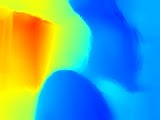
\includegraphics[width=0.8\linewidth]{images/depth_full-depth-image}
        \caption{Full Depth API depth image}
    \end{subfigure}%
    \begin{subfigure}[b]{0.4\textwidth}
        \centering
        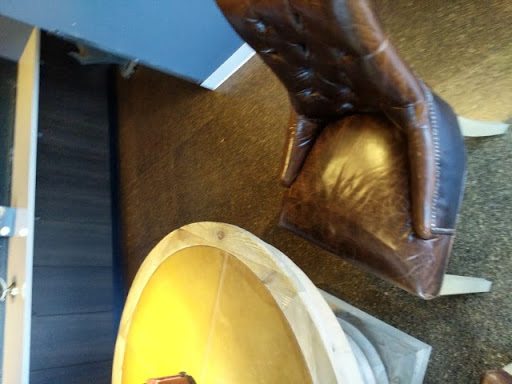
\includegraphics[width=0.8\linewidth]{images/depth_camera-image}
        \caption{Camera image}
    \end{subfigure}%

    % Optional: Adjust or remove vertical spacing between the rows
    \vspace{0.5em}

    % Second row
    \begin{subfigure}[b]{0.4\textwidth}
        \centering
        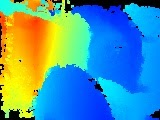
\includegraphics[width=0.8\linewidth]{images/depth_raw-depth-image}
        \caption{Raw Depth API depth image}
    \end{subfigure}%
    \begin{subfigure}[b]{0.4\textwidth}
        \centering
        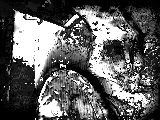
\includegraphics[width=0.8\linewidth]{images/depth_raw-depth-confidence-image}
        \caption{Raw Depth API confidence image}
    \end{subfigure}%

    \caption{Full Depth vs. Raw Depth. Source: \cite{google_llc_arcore_doc}}
    \label{fig:depth-api-images}
\end{figure}

Both Depth APIs have their use cases --
the Full Depth API is preferred in cases where it is crucial to have a depth value for every pixel, such as calculating if an object should be occluded by the scene in an AR application,
while the Raw Depth API is preferred if accuracy of the depth information is crucial.
As accuracy is crucial for primitive detection and depth information for every pixel is not required, the Raw Depth API is used in this thesis.

\subsection{Technical Background: Depth From Motion}\label{sec:technical-background-depth-from-motion}
Depth from motion is a technique developed by Google that estimates depth information from a sequence of monocular camera images
and is used by the ARCore Depth API to provide depth information.
Its primary purpose is to enable AR applications that rely on depth information on devices lacking a dedicated depth sensor or multiple cameras.
This sections provides a brief overview of the workings of the Depth from Motion system by ~\parencite{valentin_depth_2018}.

\begin{figure}[ht!]
    \centering
    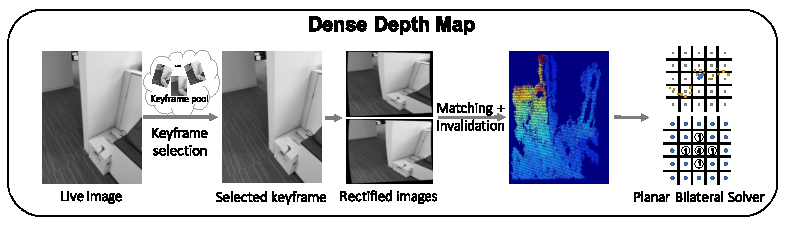
\includegraphics[width=\linewidth]{images/DepthFromMotion}
    \caption{Overview of the Depth from Motion System. Source: \cite{valentin_depth_2018}}
\end{figure}
When users move their smartphones, the system uses ARCore's visual-inertial odometry (VIO)
to determine its position and orientation in six dimensions (6DoF): up/down, left/right, forward/backward, and tilt/swivel/rotate.
After activating tracking and acquiring the most recent camera image (in black and white for faster processing),
a reference image or keyframe from the past is chosen to compare with the current image.

A process known as polar rectification then aligns the keyframe and current frame onto the same plane based on their differences in position and orientation.
This alignment simplifies the process of finding matching points in both images by focusing on comparable horizontal lines.

Next, they use an image correspondence algorithm to identify matching points,
which generates disparity maps that indicate the positional differences between matched points in the two images.
As scenes may contain low textured objects or repetitive patterns which can lead to incorrect matches,
they use an invalidation step, which removes points that are likely to be incorrect matches.
This step also provides a confidence value, which is later used in the interpolation step.
Triangulation is used to compute a sparse depth map based on the disparity maps.

The missing values in the sparse depth maps are then interpolated using a variation of an algorithm called the bilateral solver (see figure~\ref{fig:depth-from-motion-interpolation}),
which yields an intermediate data structure known as a bilateral depth grid.
This grid is a structured representation of depth information that can be converted into a full depth map on demand,
assessable through the Full Depth API\@.

\begin{figure}[ht!]

    \centering
    \begin{subfigure}[b]{0.4\textwidth}
        \centering
        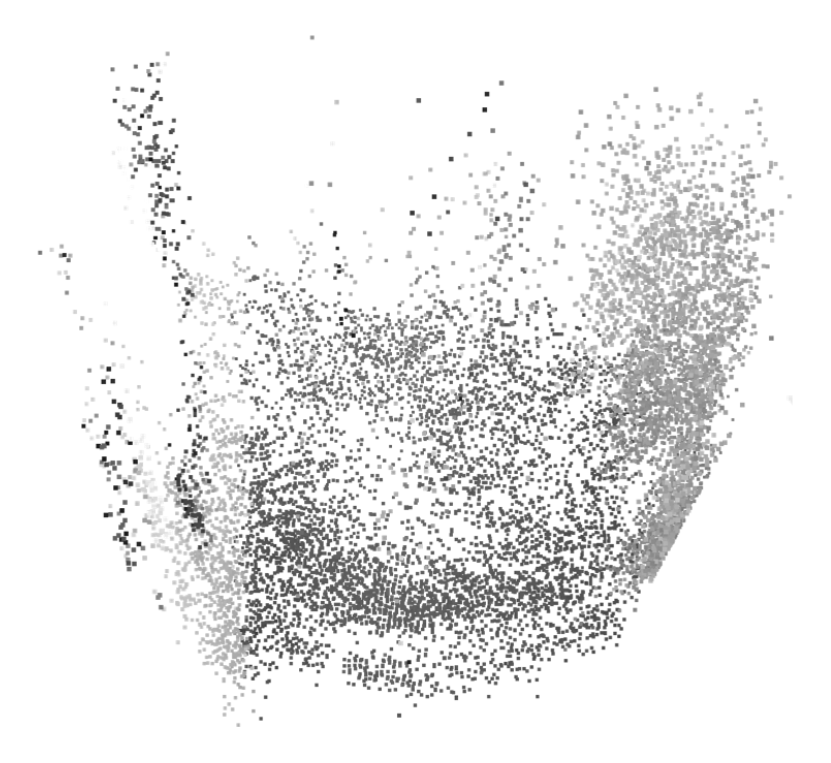
\includegraphics[width=\linewidth]{images/DepthFromMotionBilateral1}
        \caption{Raw point cloud}
    \end{subfigure}%
    \begin{subfigure}[b]{0.4\textwidth}
        \centering
        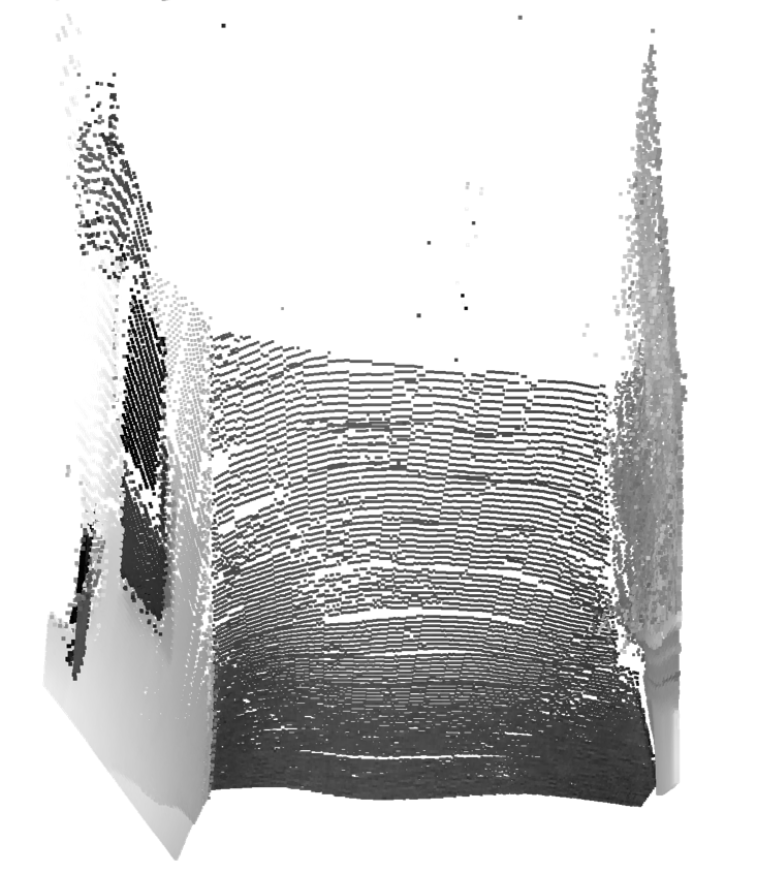
\includegraphics[width=\linewidth]{images/DepthFromMotionBilateral2}
        \caption{Interpolated}
    \end{subfigure}%
    \caption{Interpolation with Bilateral Solver. Source: \cite{valentin_depth_2018}}
    \label{fig:depth-from-motion-interpolation}
\end{figure}

From the paper it is unclear, which part of the pipeline are omitted in the Raw Depth API,
but it is reasonable to assume that the Raw Depth API accesses the sparse depth map and confidence values before the interpolation step.


\section{Building the Point Cloud}\label{sec:building-the-point-cloud}
With the depth image and confidence image collected from the Raw Depth API,
the next step is to convert the depth image into a point cloud, as RANSAC is a point-based algorithm.
The process consists of three steps:
\begin{enumerate}
    \item Filtering low confidence points
    \item Transforming depth image pixels to world coordinate points
    \item Inserting new points into the point cloud
\end{enumerate}

\subsection{Filtering Low Confidence Points}
The Raw Depth API provides a confidence image that indicates the reliability of the depth information for each pixel.
To improve the accuracy of the point cloud, points with low confidence are filtered out.
A threshold value is set, below which points are discarded.
Filtering out low confidence points early in the pipeline also improves performance,
as fewer points need to be processed in the following steps.

\subsection{Transforming Depth Image Pixels to World Coordinate Points}
The Depth API provides depth images where each pixel holds the distance from the camera in millimeters.
Before inserting points into the point cloud, the pixel values of the depth image
first need to be converted into 3-dimensional coordinates relative to a fixed origin in the world.
This section will first provide a brief overview of the mathematical concepts required to understand the transformation process.
Then, the process of transforming a point from the depth image into world space will be explained.

%To convert the point into world coordinates, first the camera intrinsics are used to
%project the point into camera space.
%Then, the model matrix is used to transform the point into world space.
%\parencite{google_llc_codelab_raw_depth,google_llc_arcore_doc}

\subsubsection{Transformations}

In computer graphics matrices are used to represent geometric transformations like translation, scaling, rotation,
shearing, reflection and projection.
While it is out of scope to cover all of these transformations in detail,
this section will use the example of the translation to explain the concepts of
transformations and homogenous coordinates based on~\cite{dorner_virtual_2019}.


%TODO Homogenous coordinates explaition
%which are an extension of the Cartesian coordinate system.
%In homogeneous coordinates, each point in 3D space is represented by four coordinates instead of three: $(x, y, z, w)$.

To apply transformations to a point, the points is represented in homogenous coordinates,
which is a 4x1 matrix with the fourth $w$ element set to 1.

\begin{equation}
    p = \begin{bmatrix}
            w \cdot x \\
            w \cdot y \\
            w \cdot z \\
            w
    \end{bmatrix}
\end{equation}

The homogenous coordinates are then multiplied with a transformation matrix $M$ to apply the transformation.
\begin{equation}
    p' = M \cdot p
\end{equation}
In the case of a translation, the translation matrix is a 4x4 matrix with the translation vector $t$ as the fourth column.
\begin{equation}
    p' = \begin{bmatrix}
             1 & 0 & 0 & t_x \\
             0 & 1 & 0 & t_y \\
             0 & 0 & 1 & t_z \\
             0 & 0 & 0 & 1
    \end{bmatrix} \cdot \begin{bmatrix}
                            w \cdot x \\
                            w \cdot y \\
                            w \cdot z \\
                            w
    \end{bmatrix} = \begin{bmatrix}
                        w \cdot (x + t_x) \\
                        w \cdot (y + t_y) \\
                        w \cdot (z + t_z) \\
                        w
    \end{bmatrix}
\end{equation}

Note that transformation can also effect the fourth element $w$, as later explained in the section about perspective projection.
To account for this, the resulting matrix is then divided by the fourth element $w$.
The cartesian coordinates of the point are then the first three elements of the resulting matrix.

One advantage of using matrices to represent transformations is that multiple transformations can be combined by
multiplying the transformation matrices.
The resulting matrix will then apply all transformations in the order they were multiplied.
\begin{equation}
    p' = (M_n \cdots M_3 \cdot M_2 \cdot M_1) \cdot p
\end{equation}
If multiple transformations were to be applied to thousands of points,
it would be more efficient to multiply the transformation matrices once and then apply the resulting matrix to all points~\cite{de_vries_learn_2020}.
Graphics Processing Unit's (GPUs) also contain hardware implementation of 4x4 matrix operations,
which further increases the performance of matrix operations over other methods~\cite{dorner_virtual_2019}.
Transformation matrices can also be inverted ($M^{-1}$) to apply the inverse transformation, or in other words 'undo' the transformation~\cite{dorner_virtual_2019}.

\subsubsection{Coordinate Systems and Basis Change}

Different coordinate systems, also known as spaces~\cite{de_vries_learn_2020}, are commonly utilized to represent points
in space, allowing for simplified calculations.
To illustrate this, consider a camera inside a moving car, filming a person inside the car.
In order to implement smooth camera movement around the person,
calculations based on coordinates relative to the world (world space) would need to account for the car's movement in each frame.
By using the car's local coordinate system, where all points are relative to the clarity.~\cite{de_vries_learn_2020}

To transform points between these systems, their positions are multiplied with a corresponding transformation matrix.
To improve performance, these matrices are often combined to a singular matrix, called the MVP-Matrix,
that transforms points from local space to screen space. \cite{de_vries_learn_2020}

\begin{figure}[h!]
    \centering
    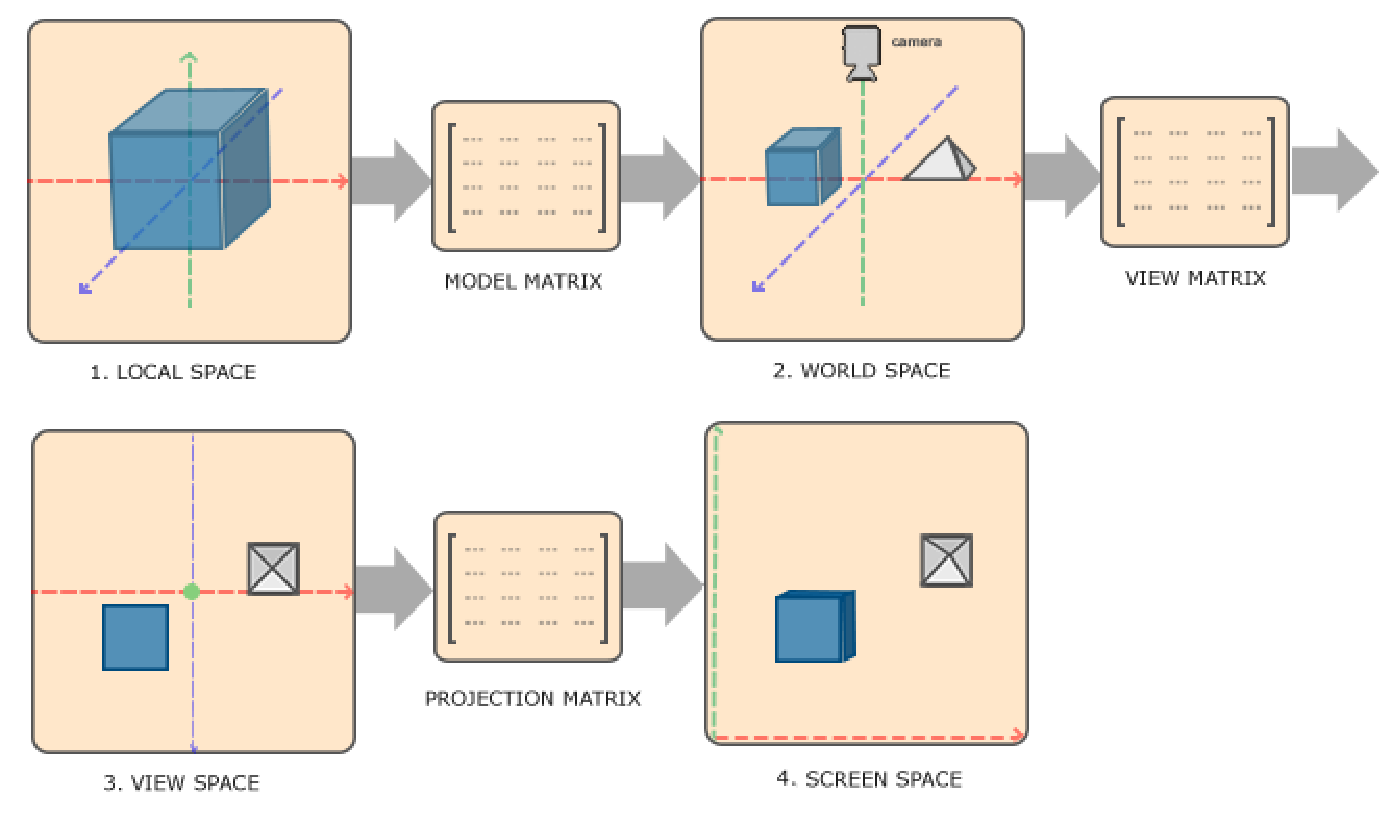
\includegraphics[width=0.85\linewidth]{images/coordinateSystemsAdjusted}
    \caption{Coordinate systems. Adjusted from \cite{de_vries_learn_2020}.}
    \label{fig:coordinate-systems}
\end{figure}

\subsubsection{Perspective Projection and Camera Intrinsics}\label{sec:perspective-projection}
In the real world, objects appear smaller the further away they are from the viewer.
The same concept applies to images captured by cameras.
To illustrate this, consider a simpel pinhole camera model, as shown in figure~\ref{fig:pinhole-camera-model}.
\begin{figure}[h!]
    \centering
    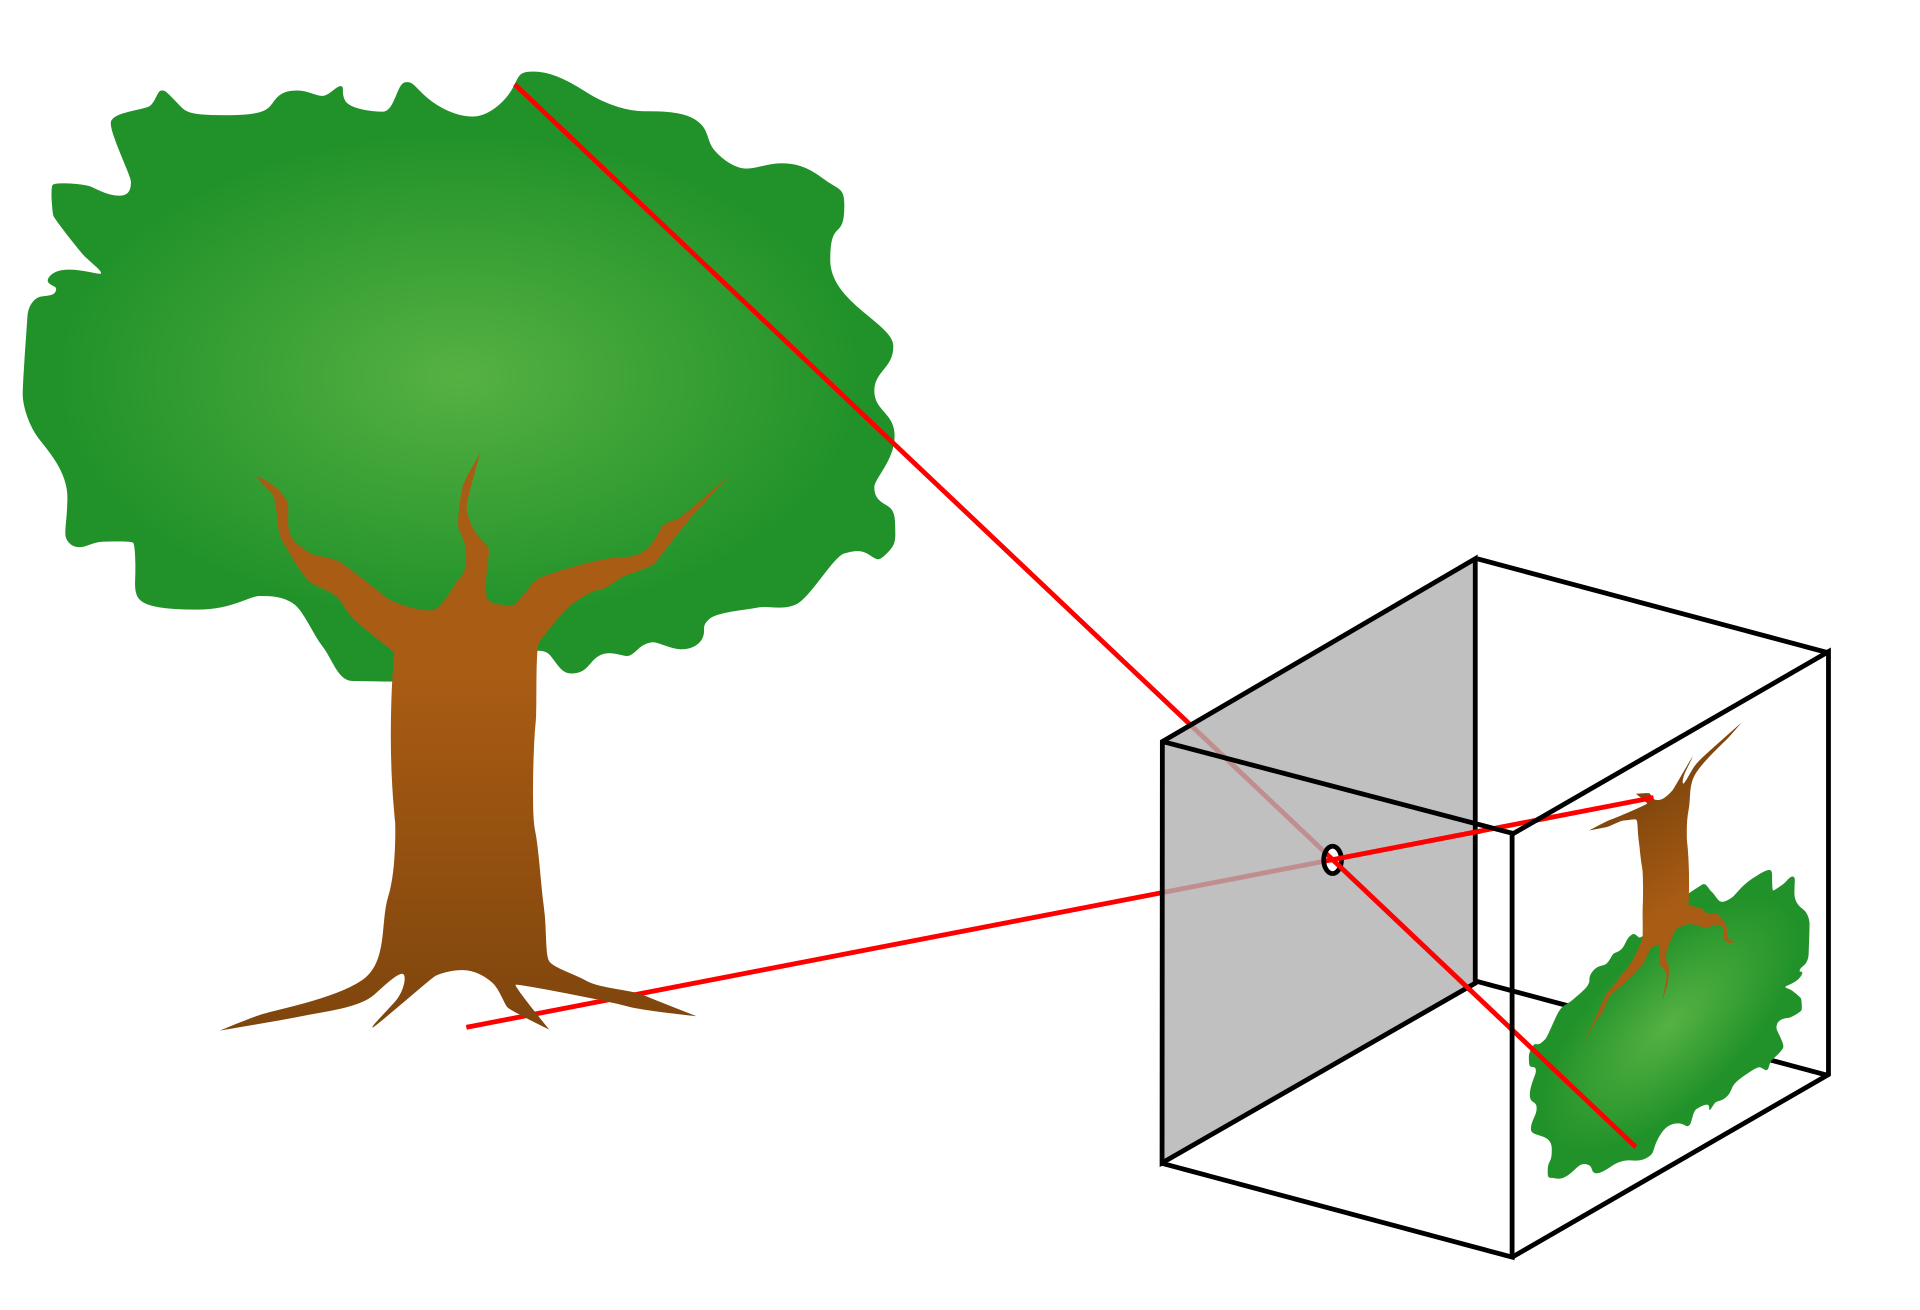
\includegraphics[width=0.45\linewidth]{images/pinhole}
    \caption{Pinhole camera model. Source: \href{https://commons.wikimedia.org/wiki/File:Pinhole-camera.svg}{Wikimedia Commons}}
    \label{fig:pinhole-camera-model}
\end{figure}
The camera is represented as a box with a small hole (aperture) on one side.
This aperture allows light rays from the scene to pass through and form an inverted image on the opposite side of the box
In the diagram, the red lines depict the light rays corresponding to the top and bottom of the tree.
The closer the tree is to the camera, the smaller it needs to be to fit inside the two rays,
or in other words to appear the same size on the image plane.
This concept is known as perspective projection and can be achieved by dividing the
$x$ and $y$ coordinates of a point by its $z$ coordinate.
During this process, the z coordinate is lost and can't be recovered. \cite{szeliski_computer_2022}
\begin{equation}
    P_s = \begin{bmatrix}
              x/z \\
              y/z \\
              1
    \end{bmatrix}
\end{equation}

This however, does not account for the geometry of the camera itself -- the camera intrinsics.
These intrinsics are a set of parameters that describe the camera's geometry and are used to calculate the projection~\cite{szeliski_computer_2022}.
The two most important parameters are the focal length $f$ and the image center $c$, as shown in figure~\ref{fig:intrinsics-3d}.

\begin{figure}[ht!]
    \centering
    \begin{subfigure}[t]{0.45\textwidth} % Adjusted from 0.4 to 0.45
        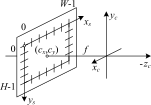
\includegraphics[width=1\linewidth]{images/intrinsics}
        \caption{Geometry of a camera with an image plane height $H$, width $W$, focal length $f$, and principal point $c$. Source: \cite{szeliski_computer_2022}}
        \label{fig:intrinsics-3d}
    \end{subfigure}%
    \hspace{0.05\textwidth} % Added space between subfigures
    \begin{subfigure}[t]{0.45\textwidth} % Adjusted from 0.4 to 0.45
        \resizebox{\linewidth}{!}{
            
\usetikzlibrary{arrows.meta}
\tikzset{
    myptr/.style={-{Stealth[scale=3]}},
}
\begin{tikzpicture}[scale=1, every node/.style={scale=0.8}, every path/.style={scale=0.7, thick}]

    % Coordinate system
    \draw[shorten >=2pt, shorten <=2pt] (0,0) -- (3,0);
    \draw[-{Stealth[round]}, shorten <=2pt] (3,0) -- (6,0) node[anchor=north] {$-z_c$};
    \draw[-{Stealth[round]}, shorten <=2pt] (0,0) -- (0,4) node[anchor=east] {$y_c$};


    % Camera
    \node[anchor=north east] at (0,0) {$C$};
    \draw (0,0) circle (2pt);
    % line from C to A
    \draw[shorten >=2pt, shorten <=2pt] (0,0) -- (3,1.5);
    \draw (5,2.5) circle (2pt);
    \node[anchor=south east] at (3,1.5) {$a$};
    \draw (3,1.5) circle (2pt);
    \draw[shorten >=2pt, shorten <=2pt] (3,1.5) -- (5,2.5);
    \node[anchor=south west] at (5,2.5) {$A$};
    \draw (5,2.5) circle (2pt);

    % x line
    \draw[dashed, shorten >=2pt] (5,0) -- node[right] {$z$} (5,2.5);
    % y line
    \draw[dashed, shorten >=2pt] (0,2.5) -- node[above] {$y$} (5,2.5);

    % f line
    \draw[<->] (3,-0.25) -- node[below] {$f$} (0,-0.25);
    % z line
    % \draw[<->] (0,-0.2) -- node[below, xshift=12mm] {$z$} (5,-0.2);


    % Image plane
    \draw[shorten <=2pt, shorten >=2pt] (3,0) -- (3,1.5);
    \draw[shorten <=2pt] (3,1.5) -- (3,3);

%    principal point
    \draw (3,0) circle (2pt);
    \node[anchor=north west] at (3,0)  {$c$};

    % fY/Z line
    \draw[<->] (3.25,0) -- node[right] {$f\frac{y}{z}$} (3.25,1.5);
%    \draw[dashed] (2.75, 1.5) -- (3.5, 1.5);


\end{tikzpicture}
        }
        \caption{Projection of an observed point $A$ onto the image plane in the $y$-direction. Based on~\cite{kris_kitani_computer_2017} and~\cite{google_llc_arcore_doc}}
        \label{fig:intrinsics-2d}
    \end{subfigure}%
    \caption{Camera intrinsics}
    \label{fig:intrinsics}
\end{figure}

The focal length $f$ is the distance between the image plane and the aperture of the camera.
The image center $c$ (also called principal point) is the point where the principal axis $z_c$
intersects the image plane, denoted in pixel coordinates.
Figure~\ref{fig:intrinsics-2d} shows the projection of an observed point $A$ onto the image plane.
Note that the image plane is displayed in the $-z_c$ direction, as opposed to $+z_c$ direction.
It shows how the focal length $f$ affects the $y$-coordinate of the projected point.
\cite{szeliski_computer_2022, google_llc_arcore_doc, kris_kitani_computer_2017}
This can be simulated by using ones fingers to form a square that represents a virtual
image plane and moving it closer or farther to the eye.
The farther away the square is (higher focal length), the less field of view the square covers.

Mathematically, the projection is often represented as a matrix, called the calibration matrix
\begin{equation}
    K = \begin{bmatrix}
            f_x & 0   & c_x \\
            0   & f_y & c_y \\
            0   & 0   & 1
    \end{bmatrix}
\end{equation}
with independent focal lengths $f_x$ and $f_y$ to account for aspect ratios other than 1:1.
As different focal lengths in each dimension do not reflect the real geometry of a camera,
a more intuitive way to understand different focal lengths can be used by introducing the aspect ratio a:
\begin{equation}
    K = \begin{bmatrix}
            f & 0  & c_x \\
            0 & af & c_y \\
            0 & 0  & 1
    \end{bmatrix}
\end{equation}
\parencite{szeliski_computer_2022}




\subsubsection{Applying the transformation to the depth pixels}
With the mathematical concepts clarified, the transformation of depth image pixels into world space can be explained.
First, it is necessary to understand how the depth values are represented in the depth image.

In terms of coordinate systems, the depth values are in screen space, as shown in figure~\ref{fig:coordinate-systems}.
To convert these points into world space, the transformations need to be applied backwards:
\begin{enumerate}
    \item From screen space to view space (`unprojecting`)
    \item From view space to world space
\end{enumerate}
%`Unprojecting` the pixel from screen space to view space and then to world space is required.
%Note that clip space is not applicable here, as ARCore provides intrinsics in pixels, not normalized device coordinates,
%thus the projection matrix directly transforms from view space to screen space.
Another way to think about this procedure is to conceptualize the unprojecting step as transforming the pixels into a local space
relative to the camera, as defined by the camera's position, up and look vector.
Then, the point is transformed from the cameras local space into world space using the cameras model matrix.
For simplicity and to avoid confusion when transforming into different directions, the latter approach is used going forward.

The first step is to unproject the pixels from screen space to the cameras local space $K_l$, as explained by~\cite{google_llc_codelab_raw_depth, google_llc_arcore_doc}.
Referring to figure~\ref{fig:intrinsics} and
"given point $A$ on the observed real-world geometry and a 2D point $a$ representing the same point in the depth image,
the value given by the Depth API at $a$ is equal to the length of $CA$ projected onto the principal axis.
This can also be referred as the z-coordinate of $A$ relative to the camera origin $C$."~\parencite{google_llc_arcore_doc}

Using the camera intrinsics, the depth value is transformed to the local space relative to the camera $K_l$.
The camera intrinsics can be retrieved from the API using the method \texttt{frame.getCamera().getTextureIntrinsics()}.
However, this method returns the intrinsics of the camera image, which differs from the depth image, as the depth image usually has a lower resolution.
To calculate the focal length $f$ and camera center $c$ from the provided intrinsics $K$, depth image $D$ and camera image dimensions $x_{Dim}, y_{Dim}$,
the provided focal length and principal point are scaled by the ratio of the dimensions of the depth image and the camera image:
\begin{equation}
    S = \begin{bmatrix}
            \frac{\dim_x(D)}{x_{Dim}} & 0\\[8pt]
            0                         & \frac{\dim_y(D)}{y_{Dim}}
    \end{bmatrix}\\
    f = S \cdot K_f \\
    c = S \cdot K_c
\end{equation}

These values are then used to unproject the point into local space relative to the camera $K_l$ using the equation
\begin{equation}
    p_l = \begin{pmatrix}
              d \cdot (x - c_x) / f_x \\
              d \cdot (c_y - y) / f_y \\
              -d                      \\
              1
    \end{pmatrix}
\end{equation}
as evident from figure~\ref{fig:intrinsics}.

As the resulting point is in a local space relative to the camera $K_l$, it needs to be transformed into world space $K_w$.
To transform it into world space, the camera pose is retrieved and converted to a matrix:
\texttt{cameraPoseAnchor.getPose().toMatrix(modelMatrix, 0)}.
By multiplying the model matrix $T_{wl}$ with $p_l$, the point is transformed into world space.
\begin{equation}
    p_w = T_{wl} \cdot p_l
\end{equation}

\subsection{Inserting New Points into the Point Cloud}\label{subsec:inserting-new-points-into-the-point-cloud}

With all pixels from the depth image transformed to world coordinates, the final step involves adding these points to the point cloud.
However, simply storing a list of all points and appending new data to it is not feasible.
As a new depth image is captured every frame, the number of points would grow endlessly.
This approach would also result in a massive number of points representing the same point on real-world geometry,
but with slightly different position values,
as subsequent depth images will show the same real-world geometry from different angles, with depth values varying slightly.
To address this issue, a spatial data structure that partitions the space into smaller regions and
allows to store only one point per region can be used.
One possible approach is to use a three-dimensional grid, where each cell represents a region in space.
Alternatively, a more advanced approach involves utilizing a spatial data structure such as an octree,
which can provide improved performance.

\begin{figure}[h]
    \centering
    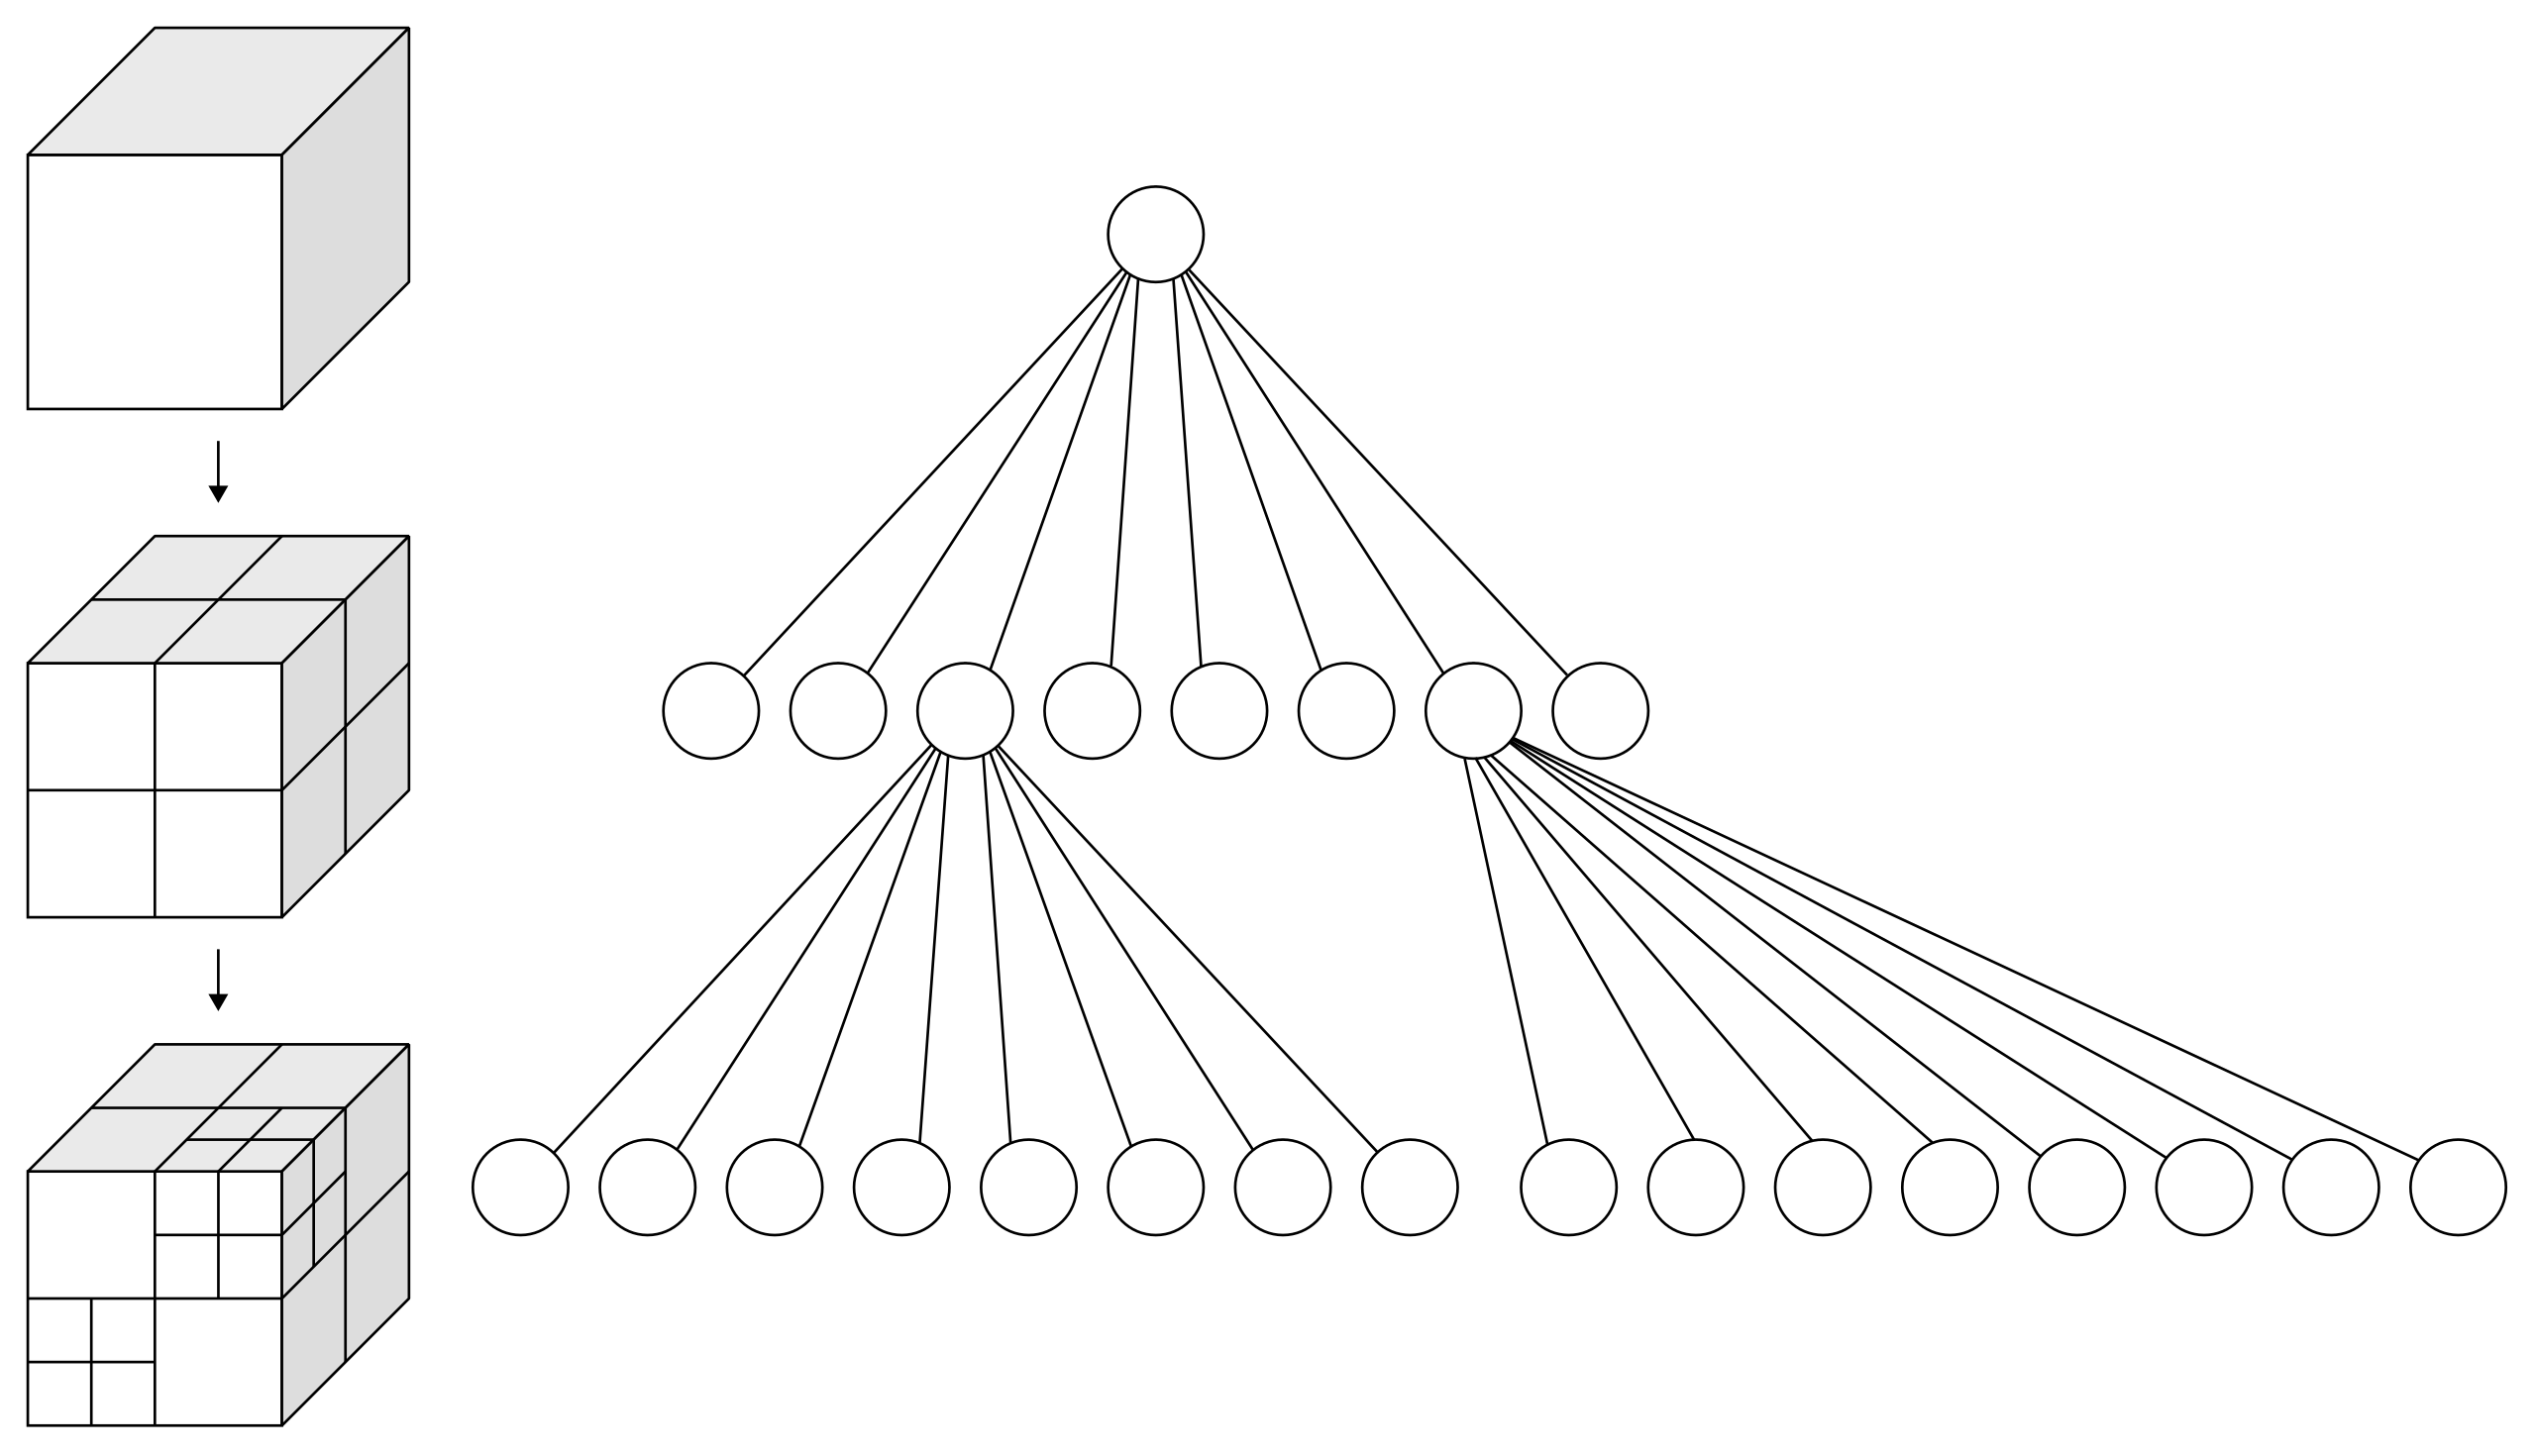
\includegraphics[width=0.65\textwidth]{images/octree}
    \caption{Octree. Source: \href{https://commons.wikimedia.org/wiki/File:Octree2.svg}{Wikimedia Commons}}
    \label{fig:octrree}
\end{figure}
\paragraph{Octree}
An octree is a spatial tree data structure where each node has exactly eight children.
The tree can be used to sparsely partition three-dimensional space into smaller cubes and allows for efficient
insertion and traversal in logarithmic time.
"For the definition a simple recursive splitting of [cubes] is continued until there is only one point in a [cube]."
\parencite{gabriel_zachmann_geometric_2002}

\subsubsection{Fixed Depth Octree}
A straightforward approach to utilize an octree for point cloud storage is to use a variation of the octree with a fixed depth.
Points are always inserted at the defined depth of the tree, creating all nodes up to that depth if they do not yet exist.
The center coordinate of the leaf node can then be inferred as the point in space,
thus saving the coordinates of the point explicitly is not required.
Instead, to find the coordinates of a given node, the tree needs to be traversed while keeping track of
the extent and center coordinate of the current node.
This approach will naturally provide quantization of the point cloud, with the resolution of the point cloud
determined by the depth of the octree and extend of the root.
This is functionally equal to a three-dimensional grid,
but with the advantage of logarithmic time complexity for insertion and traversal.
Using this approach, duplicate points are removed and adjusting the resolution of the octree
allows for fine-tuning of the threshold distance between points under which points are considered duplicates.

One advantage of an octree with a fixed width is simplicity, as points are always inserted at the same depth and deletion of points is not required.
The biggest drawback is that the resolution of the point cloud is fixed and needs to be chosen beforehand.
As the accuracy of the depth values differs based on conditions like lighting and texture of the captured surface,
it is difficult to choose a fixed resolution that works for all values.

%When using a resolution that is too high, some surfaces might be detected as multiple surfaces instead of one.
%This is due to the same point being detected multiple times with slightly different depth values.
%If the uncertainty of the depth data is too high for the chosen resolution,
%points representing the same point in space will be added to neighboring cells of the octree.
%In the case of planes, this will lead to points in multiple cells across the normal of the plane,
%(increasing the thickness of the plane).

Quantization might also lead to worse detection results for surface that do not align with the axis of the octree.
For example, a plane that is tilted by a couple of degrees will lead to aliasing,
meaning that the distance between the points and the fitted plane will vary across the plane, as demonstrated in figure~\ref{fig:aliasing}.
\begin{figure}[h!]
    \centering
    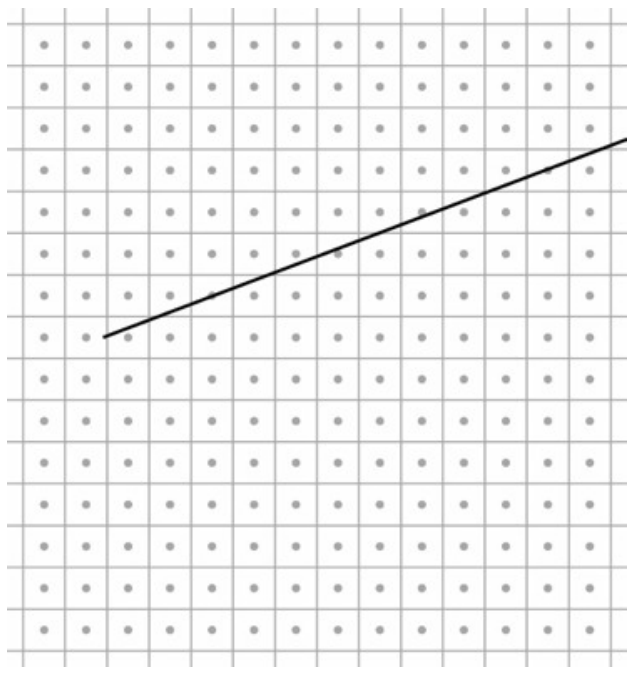
\includegraphics[width=0.35\linewidth]{images/aliasing}
    \caption{TODO better image, Example of aliasing, distance between the line and cell centers varies across cells}
    \label{fig:aliasing}
\end{figure}


\subsubsection{Octree with Neighborhood}

To improve upon the fixed depth octree, the actual point coordinates can be saved in a given node of the octree.
%Another way to use an octree for point cloud storage is to the point coordinates and its data is saved in the leaf nodes of the octree.
Furthermore, the confidence value can also be stored, in order to determine how accurate it's position is.
This allows to improve the accuracy of the data as new, higher confidence data arrives.
In order to achieve this, custom logic on inserting new points is required:
When inserting a new point with a certain confidence value, a range query with a radius calculated from the confidence value
is performed to find all nodes within a certain distance of the point to be inserted.
\begin{itemize}
\item If no node is found, a new leaf node is created and the point is inserted.
\item If a node is found with a lower confidence value, the new point is inserted and the old node is removed.
\item If a node is found with a higher confidence value, the new point is not inserted and discarded.
\end{itemize}
Using this approach, duplicate points are removed and adjusting the multiplier for the radius of the range query
allows for fine-tuning of the threshold under which points are considered duplicates.
From here on, this approach will be referred to as the \textit{Epsilon Octree}.

\paragraph{Range Query}
To check if an octree node, which is an axis-aligned bounding box (AABB) with equal sides, and a sphere intersect,
the square distance between the center of the sphere and the closest point on the AABB is calculated.
If the square distance is smaller than the square of the radius of the sphere, the sphere and the AABB intersect.

Calculating the square distance between a sphere and the closest point on the AABB can be achieved by summing up the
squared distance in each dimension:
If the sphere's center is outside the extent of the box on a given axis,
the distance is the amount by which it exceeds the box's boundary; otherwise, the distance is zero.
In $n$ dimensions, this can be expressed as
\begin{equation}
    d^2 = \sum_{i=1}^{n} \left\{
    \begin{array}{ll}
    (C_i - B_i - s)
        ^2                & \text{if } C_i > (B_i + s) \\
        (C_i - B_i + s)^2 & \text{if } C_i < (B_i - s) \\
        0                 & \text{otherwise}
    \end{array}
    \right\}
\end{equation}
where $C$ is the center of the sphere, $B$ is the center of the AABB, and $s$ is the half-size of the AABB\@.
\parencite{glassner_graphics_1994}

\paragraph{Deleting nodes}
Deleting nodes from an octree is a non-trivial task~\parencite{samet_design_1989, finkel_quad_1974}, as it may require restructuring the tree to maintain the octree properties.
\citeauthor{finkel_quad_1974}~\parencite{finkel_quad_1974} suggest reinserting all child nodes of the deleted node,
while~\cite{samet_deletion_1980} propose a more efficient method that tries to replace the deleted node with a suited node, such that the octree properties are maintained.
For simplicity, the first approach is used.
In addition, an optimization is made:
As nodes are only deleted when a new point is inserted with a higher confidence value,
it is possible to simply update the old node with the new position, in case the octree properties are not violated.
This is the case when the new point is within the same cell as the old point.
The tree is first traversed once to find the node that needs to be deleted.
If the node is in the same cell as the new point to be inserted, the old node is updated with the data of the new point.
Otherwise, the old node is deleted as by~\cite{finkel_quad_1974} and the new point is inserted.

\section{Detecting Primitives using RANSAC}\label{sec:detecting-primitives-using-ransac}

To detect primitives in the point cloud, the Random Sample Consensus (RANSAC) algorithm is used,
as discussed in section~\ref{sec:choosing-an-algorithm}.
As~\cite{kaiser_survey_2019} considers~\parencite{schnabel_efficient_2007} to be the reference implementation of RANSAC
and its code is publicly available in C\texttt{++}, it will be used in this thesis.

\subsection{Schnabel's Efficient RANSAC Algorithm}\label{subsec:schnabels-efficient-ransac-algorithm}
\citeauthor{schnabel_efficient_2007}~\cite{schnabel_efficient_2007} extended the RANSAC algorithm to be more efficient
and robust for detecting primitives.
Their approach is specifically designed for detecting planes, spheres, cylinders, cones and tori in 3D point clouds.
The key improvements over the original RANSAC method are in the following areas:
\begin{itemize}
    \item \textbf{Sampling strategy}: "Since shapes are local phenomena, the a priori probability that two points belong to the same shape is higher the smaller the distance between the points"~\parencite{schnabel_efficient_2007}.
    To take advantage of this fact, they employed non-uniform sampling based on locality, which increases the probability of selecting points that belong to the same shape.
    They provide an example of the magnitude of this improvement: For a point cloud consisting of 341,587 points that contains a cylinder with 1066 points, uniform sampling would require 151,522,829 shapes candidates to be drawn, while their method only requires 64,929 candidates.
    \item \textbf{Score function}: They introduce a scoring function that evaluates the quality of a shape candidate.
    The score function is based on 3 parameters: The support of the shape (number of inliers), the deviation of the normals and a connectivity measure, that discards shapes that are not the largest connected component on the shape.
    \item \textbf{Refitting}: After a shape is detected, they refit the shape to the inliers using a least-squares method~\cite{shakarji_least-squares_1998}, and include points that are within a certain distance of the shape to declutter the point cloud.
\end{itemize}

To find connected components in the point cloud, they use a bitmap in the parameter domain of the shape.
The parameter domain refers to a parameters defining the shape, e.g. $u, v$ for a plane.
They then set a pixel in the bitmap for each point that projects into it.
The points of the largest connected component in the bitmap are then considered inliers of the shape,
while the rest are outliers and discarded / kept in the dataset for further iterations.
Optimally, the bitmaps resolution should be set to the sampling resolution of the point cloud.
For irregularly sampled point clouds, they recommend choosing the minimal resolution that is satisfied throughout the point cloud as the bitmap resolution~\cite{schnabel_efficient_2007}.
Later on this will prove to be a challenge in combination with data from the Depth from Motion algorithm, as described in section~\ref{subsec:ransac-tests-on-real-world-data}.

The algorithm requires the following parameters to be set:
\begin{itemize}
    \item \textbf{Epsilon $\epsilon$}: The maximum distance between a point and the shape to be considered an inlier.
    \item \textbf{Bitmap Epsilon $\beta$}: The resolution of the bitmap used to determine connected shapes.
    \item \textbf{Normal threshold $\alpha$}: The maximum deviation of the normals of the points to the shape.
    \item \textbf{Minimum support $n$}: The minimum number of inliers a shape needs to have to be considered a valid shape.
    \item \textbf{Overlook probability}: The probability that a point is overlooked by the sampling strategy. A higher value increases the number of shape candidates drawn but also the probability of finding the best candidate shape.
\end{itemize}

\subsection{Wrapping C\texttt{++} Code in Java/Kotlin Using SWIG}
As the RANSAC algorithm is implemented in C\texttt{++} and the application is developed for Java/Kotlin,
the C\texttt{++} code needs to be wrapped to be used in the application.
To automatically generate the necessary code to interface with Java/Kotlin,
the Simplified Wrapper and Interface Generator (SWIG) is used.
SWIG is "a program development tool that automatically generates the bindings between C/C\texttt{++}
code and common scripting languages"~\parencite{beazley_swig_1996}.
It takes an interface file that describes the functions and classes to be wrapped as input and generates the
necessary code to interface with the target language.

An example interface file is shown in codeblock~\ref{lst:swig_interface}.
First, the module name is defined using the \texttt{\%module} directive.
Then, in a block defined by the \texttt{\%\{} and \texttt{\%\}} directives,
the C\texttt{++} code that is necessary for compilation and should be included is defined.
Finally, the \texttt{\%include} directive is used to declare all classes and functions that should be wrapped by SWIG\@.
In the case of template functions and classes, the \texttt{\%template} directive also needs to be used
to explicitly instantiate a template using a specific name.
In the example codeblock, a \texttt{std::vector<Vector3f>} is wrapped as \texttt{Vector3fVector} in the target language.

\begin{lstlisting}[caption=Example SWIG interface file, label=lst:swig_interface]
%module backend
%{
#include "math/Vector3f.h"
%}

%include "std_vector.i"
%include "math/Vector3f.h"
%template(Vector3fVector) std::vector<Vector3f>;
\end{lstlisting}

In the case of generating interfaces in Java, multiple files will be generated by SWIG\@:
\begin{itemize}
    \item \texttt{backendJNI.java} contains the Java Native Interface (JNI) function declarations (denoted by the keywords \texttt{final static native}) that are used to interface with the C\texttt{++} code
    \item \texttt{backend\_wrap.cxx} contains the native C\texttt{++} implementation of the JNI function declarations above
    \item One java file for each wrapped C\texttt{++} class that internally calls the JNI functions declared in \texttt{backendJNI.java}
\end{itemize}

\subsection{Porting the Efficient RANSAC Algorithm Library to the ARM Architecture}
%The code for~\citetitle{schnabel_efficient_2007} by \citeauthor{schnabel_efficient_2007} is implemented in C\texttt{++}
%and designed to be compiled for the x86 architecture.
%To use it on an Android device, the library needs to be compiled for the ARM architecture.
%
To compile the library for ARM, a few adjustments to the code are necessary.
The library uses the \texttt{xmmintrin.h} header file, which is an x86-specific header file
that provides access to the Streaming SIMD Extensions (SSE) instruction set. %TODO QUOTATION NEEDED
In this case it is only used to allocate and free memory using the functions \texttt{\_mm\_malloc} and \texttt{\_mm\_free}.
A conditional compilation directive is added to include the header file only if the target architecture is x86.
If the target architecture is ARM, the standard library functions \texttt{malloc} and \texttt{free} are used instead.

Furthermore, the bundled compiler used by Android Studio (clang)
is stricter than the gcc compiler and requires some minor adjustments to the code.
Most notably, the error \texttt{explicit qualification required} is fixed by adding the
\texttt{this} keyword to all member function calls.
Other adjustments include fixes like removing obsolete keywords and changing deprecated
functions of the C++ standard library with their modern counterparts.

This example illustrates that wrapping code into another architecture is not always straightforward and comes with its
own set of challenges.


\section{Rendering the Primitives}\label{sec:rendering-the-primitives}
With the primitives detected using the RANSAC algorithm, the next step is to render them in the AR scene.
This section first provides an overview of the OpenGL rendering pipeline in section~\ref{subsec:opengl-rendering-pipeline}
and the necessary steps to render the planes in section~\ref{subsec:rendering-planes}.
As planes are infinite in size, section~\ref{subsec:constraining-planes-to-the-area-where-the-points-are-located}
finally explains how to create a mesh that constrains the planes to the area where the points are located,
using the convex hull algorithm.

\subsection{OpenGL Rendering Pipeline}\label{subsec:opengl-rendering-pipeline}
This section provides an overview of the OpenGL rendering pipeline and the necessary steps to render the primitives.
Explanations are based on the book~\citetitle{de_vries_learn_2020} by \citeauthor{de_vries_learn_2020}~\parencite{de_vries_learn_2020} unless stated otherwise.

\subsubsection{Polygon Meshes}\label{subsec:polygon-meshes}

\begin{figure}[h]
    \centering
    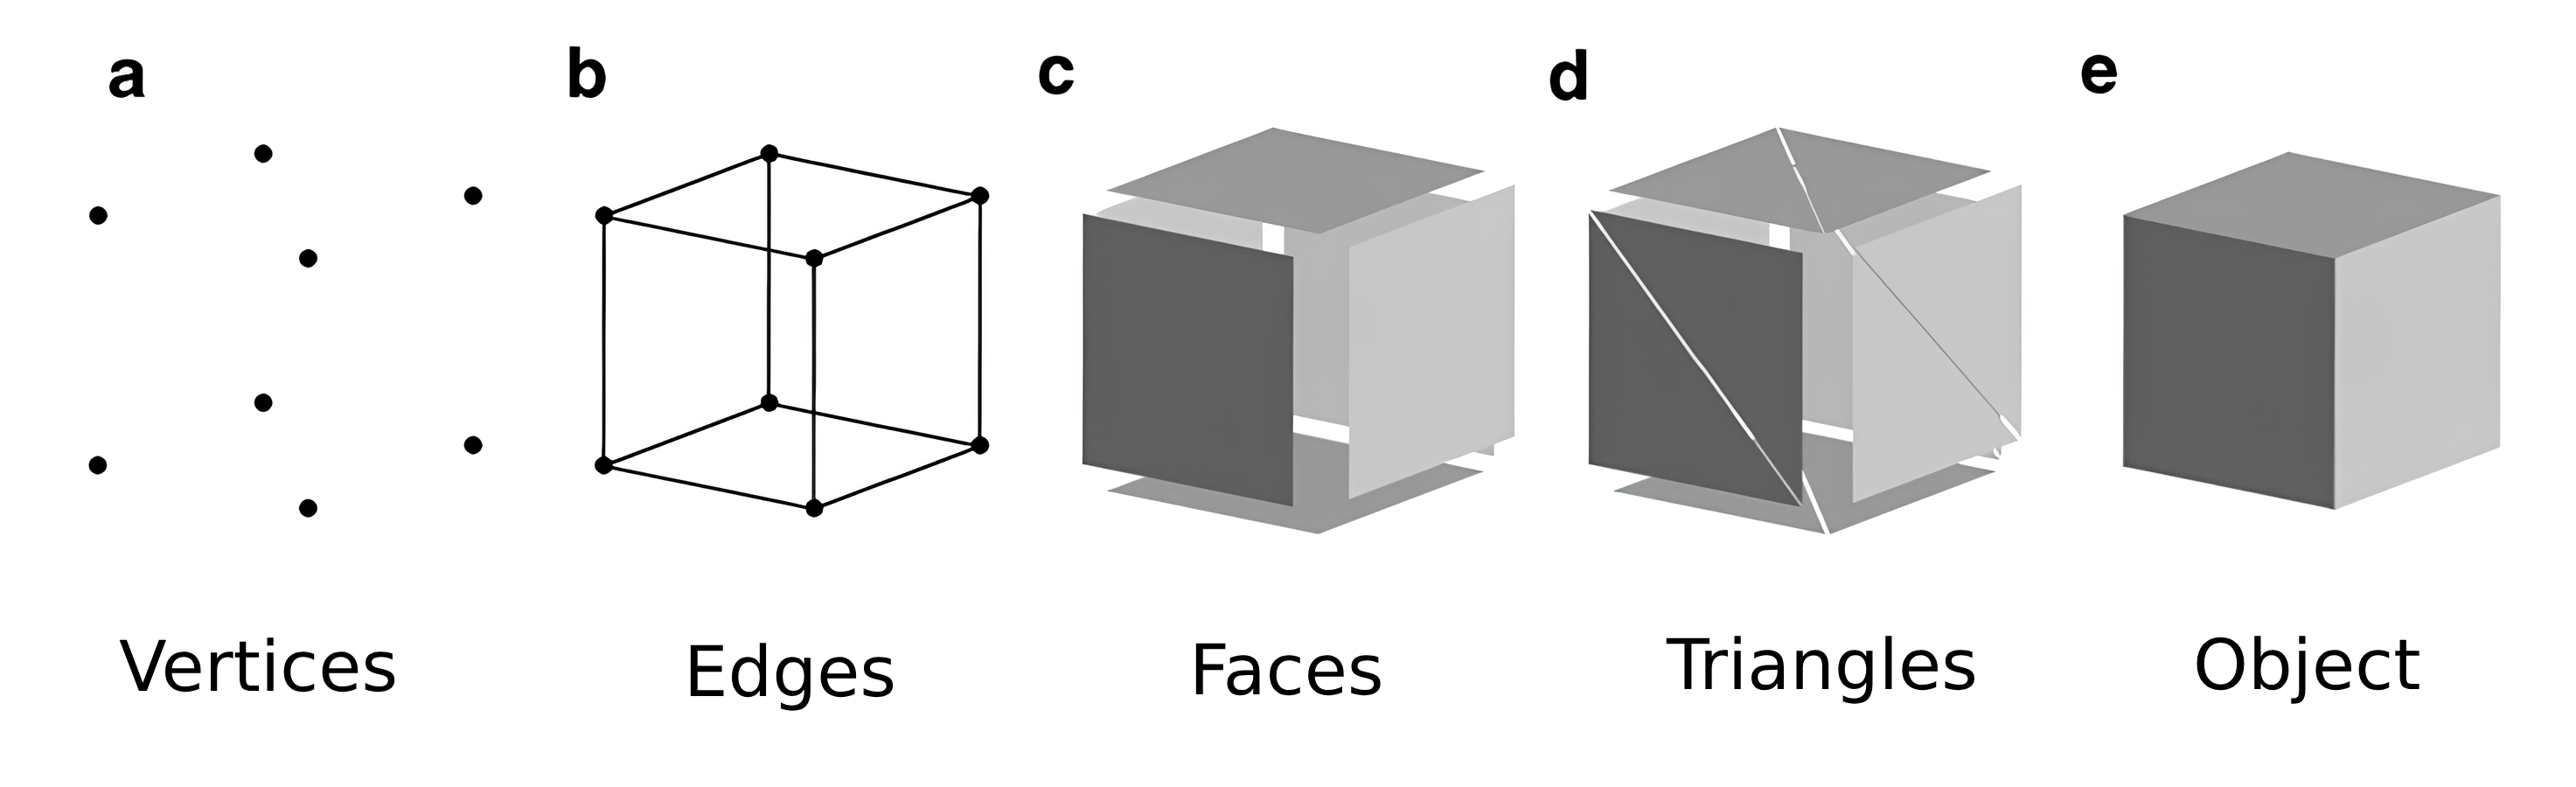
\includegraphics[width=0.70\textwidth]{images/Mesh_overview}
    \caption{Mesh overview. Source:~\cite{dorner_virtual_2019}}
    \label{fig:mesh-overview}
\end{figure}

Rendering an object is achieved by creating a polygon mesh, which is a collection of vertices that define the faces of it.
The vertices are connected by edges to form polygons, which in turn create the surface of the object.
Polygons can be of any shape, but need to be planar, meaning that all vertices lie on the same plane.
The most commonly used type of polygon is the triangle, as it is the simplest polygon that can define a surface and is guaranteed to be planar.
The graphics pipeline is also optimized for triangles, as they are easy to rasterize and interpolate.
Figure~\ref{fig:mesh-overview} shows the relationship between vertices, edges, and polygons in a mesh. \cite{dorner_virtual_2019}

Polygon meshes can be represented many ways.
The simplest representation is a list of vertices, where the vertices are stored in a specific order to form the polygons.
In OpenGL, this can be achieved by using the \texttt{glDrawArrays} function,
which takes a buffer of vertices and draws them as triangles.
However, a drawback of this approach is that vertices are often shared between multiple polygons,
resulting in redundant vertex data, as is apparent in figure~\ref{fig:mesh-overview}.
To render the cube in the figure~\ref{fig:mesh-overview}, only 8 vertices are required,
but since each of the 6 faces is rendered with two triangle,
a total of 36 vertices would be required when using this approach.~\cite{dorner_virtual_2019, de_vries_learn_2020}


\begin{figure}[h]
    \centering
    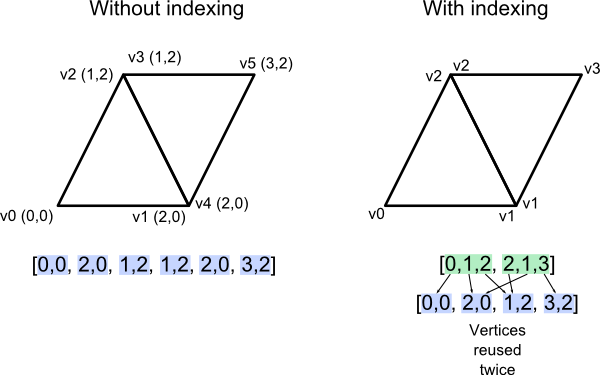
\includegraphics[width=0.60\textwidth]{images/index_buffer}
    \caption{The concept of indexing. VBO in blue, EBO in green.}
    \label{fig:index-buffer}
\end{figure}

To address this issue, a common solution is the use of an indexed face-set, which is a datastructure consisting
of two lists -- one for the vertices and one for the indices.
The vertices list contains all unique vertices of the mesh, while the indices list contains the indices of the vertices that form the polygons.
In OpenGL, the \texttt{glDrawElements} function is used to draw indexed meshes
It which requires two buffers to be bound:
The Vertex Buffer Object (VBO) for the vertices and the Element Buffer Object (EBO) for the indices.~\cite{dorner_virtual_2019, de_vries_learn_2020}
Figure~\ref{fig:index-buffer} illustrates the concept of indexing.

\subsubsection{Shaders}\label{subsec:shaders}
%here

This section provides an overview of shaders and their role in the rendering pipeline as detailed by~\cite{de_vries_learn_2020}.

Shaders are isolated programs that run on the GPU and can be used to render objects.
In OpenGL, they are written in the OpenGL Shading Language (GLSL).
Two types of shaders are required to render an object: Vertex shaders and fragment shaders.
See figure~\ref{fig:graphics-pipeline} for an overview of the graphics pipeline.
\begin{figure}[h!]
    \centering
    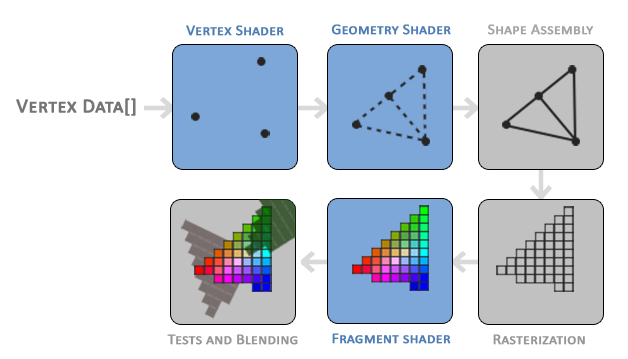
\includegraphics[width=0.70\textwidth]{images/graphics-pipeline}
    \caption{Graphics Pipeline. Blue boxes represent programmable stages. The Geometry Shader is optional and not covered in this thesis. Source:~\cite{de_vries_learn_2020}}
    \label{fig:graphics-pipeline}
\end{figure}

Vertex shaders are executed for each vertex defined in the vertex buffer, which is defined on the CPU and
passed to the GPU by copying the data to the GPU's memory, e.g.\ by using the \texttt{glBufferData} function.
This data can contain any attributes of the vertex, such as position, color, texture coordinates, or normals.
The vertex shader is then executed for each vertex and can be used to transform the vertex position between different coordinate systems,
or manipulate the vertex attributes on a per-vertex basis.
To pass data back to the pipeline, the vertex shader can define \texttt{out} variables.
In case of the vertex position, the output position is passed back to the
pipeline by assigning it to the \texttt{gl\_Position} variable using homogeneous coordinates.
OpenGL expects the vertex position to be in normalized device coordinates (NDC),
which range from -1 to 1 in all dimensions~\cite{dorner_virtual_2019}:
\begin{equation}
    (x, y, z) \in [-1, 1] \times [-1, 1] \times [-1, 1]
\end{equation}
All coordinates outside this cube are considered outside the view of the camera and subsequently clipped,
which means they will not be rendered.
Note that in other implementations, the cube might be defined with $z \in [0, 1]$.

The graphics pipline then uses the NDC and performs the perspective divide,
which divides the $x$, $y$, and $z$ coordinates by the $w$ coordinate of the homogenous coordinates,
resulting in a reduction of dimension from 4 to 3.
Then, the viewport transformation, which maps the NDC to screen space,
parameterized by the screen width and height in pixels, is performed.
Rasterization and interpolation of the vertex positions alongside all other vertex attributes
is then performed across the primitive.
The resulting elements are called fragments.
The fragment shader is then executed for each rasterized fragment of the primitive and is expected to
output a color by setting the \texttt{out vec4 FragColor} variable.
The screen position of the fragment and all variables that were passed as \texttt{out} from the
vertex shader can also be accessed in the fragment shader, with their values interpolated across the primitive.
This allows for smooth color transitions or texture mapping across the primitive.
Before the final color is written to the framebuffer,
a depth test is performed to determine if the fragment is visible or covered by fragments from other primitives,
in which case it is discarded.


\subsubsection{Perspective Projection in OpenGL}

As discussed in section~\ref{sec:perspective-projection}, perspective projection is used
to simulate the effect of objects appearing smaller the further away they are from the viewer.
This transformation from 3D space to a 2D projection is handled by a projection matrix.
In OpenGL rendering however, the projection matrix does not directly transform from view-space to screen-space.
Instead, an intermediate coordinate system known as clip space is introduced, as shown in figure~\ref{fig:coordinate-systems-with-clip-space}.
\begin{figure}[h!]
    \centering
    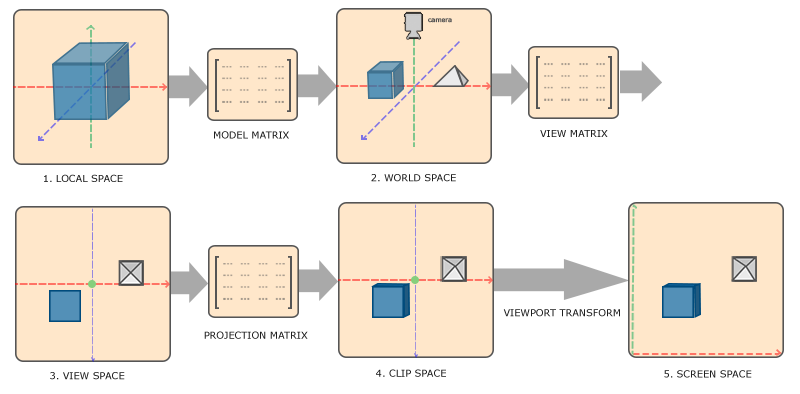
\includegraphics[width=0.85\linewidth]{images/coordinate_systems}
    \caption{Extension of coordinate systems by clip space. Source: \cite{de_vries_learn_2020}}
    \label{fig:coordinate-systems-with-clip-space}
\end{figure}
Coordinates in clip space are in normalized device coordinates (NDC), which is a cube
with coordinates ranging from -1 to 1 in all dimensions, as discussed in the previous section.

%A vertex shader can be used to transform the vertices from model space to screen space using the
%model, view, and projection matrices.
%To achieve this, the Model-View-Projection matrix (MVP) matrix can be passed as a \textit{uniform} to the vertex shader,
%which means it is the same for all vertices.
%The MVP matrix is the result of multiplying the model matrix, view matrix, and projection matrix.
%As the MVP matrix is the same for all vertices of an object, it can be calculated on the CPU and passed to the GPU as a uniform.
%The vertex position is then multiplied by the MVP matrix to transform it into clip space.

The projection matrix defines a frustum, which, depending on the projection type, can be a truncated pyramid or a cube,
that defines the volume of space visible through the camera lens.
In the case of the perspective projection, the frustum is a truncated pyramid, as shown in figure~\ref{fig:perspective}.
The parameters of the frustum are defined by the field of view, aspect ratio, and near and far clipping planes.
\begin{figure}[h!]
    \centering
    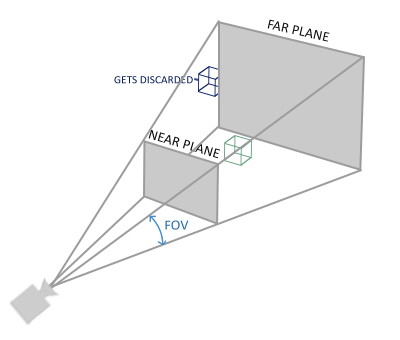
\includegraphics[width=0.50\textwidth]{images/perspective}
    \caption{Frustrum defined by perspective projection. Source: \cite{de_vries_learn_2020}}
    \label{fig:perspective}
\end{figure}
Multiplication of the vertex position with the projection matrix transforms the vertex into clip space.
"The projection matrix [\ldots] also manipulates the w value of each vertex coordinate in such a way
that the further away a vertex coordinate is from the viewer, the higher this w component becomes"~\parencite{de_vries_learn_2020}.
When the coordinates are later divided by $w$ in the perspective divide,
it results in the desired perspective scaling effect.
Points closer to the viewer have a smaller $w$ and are less affected by the divide,
while points further away have a larger $w$ and are reduced in size more significantly.


\subsection{Rendering Planes}\label{subsec:rendering-planes}
The RANSAC algorithm provides the parameterization of any detected plane using a normal vector $n$ and the point $p$ relative the worlds origin.
Using OpenGL, a plane can be rendered by creating two triangles composed of 3 vertices each, with two corner vertices shared between the triangles.
To render a plane from the parameterization, one can first find two arbitrary vectors $u$ and $v$
that are perpendicular to each-other and to the normal vector $n$.
Using $u$ and $v$, the four corner vertices of the plane can then be calculated by adding and subtracting $u * size / 2$ and $v * size / 2$ from the point $p$.

\paragraph{Calculating an Arbitrary Perpendicular Vector}
The cross product of two vectors $a$ and $b$ is a vector that is perpendicular to both $a$ and $b$,
as long as $a$ and $b$ are not parallel.
To calculate an arbitrary perpendicular vector to a given vector $n$, one can use any of the 3 basis vectors ${b_1}$, ${b_2}$, and ${b_3}$.
Choosing any of the basis vectors that is not parallel to $n$ will result in a perpendicular vector.
To minimize floating point errors, which are largest for planes where $n$ almost aligns with the chosen basis vector,
the basis vector with the smallest dot product with $n$ can be chosen.
The normalized cross product of two vectors $n$ and $b_{smallest}$ then yields a perpendicular vector to $n$.

\begin{figure}[ht!]
    \centering
    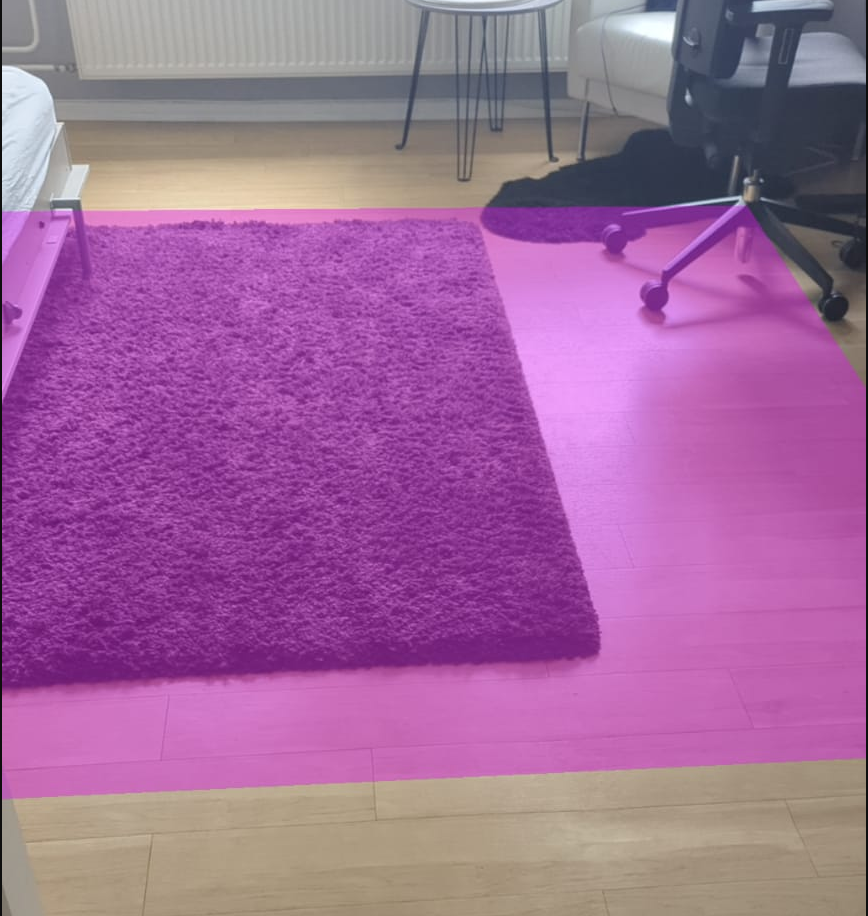
\includegraphics[width=0.5\linewidth]{images/renderedPlane}
    \caption{Rendered RANSAC plane with size of 2*2m}
\end{figure}

\subsection{Constraining Planes to the Area Where the Points Are Located}\label{subsec:constraining-planes-to-the-area-where-the-points-are-located}

\begin{figure}[ht!]
    \centering
    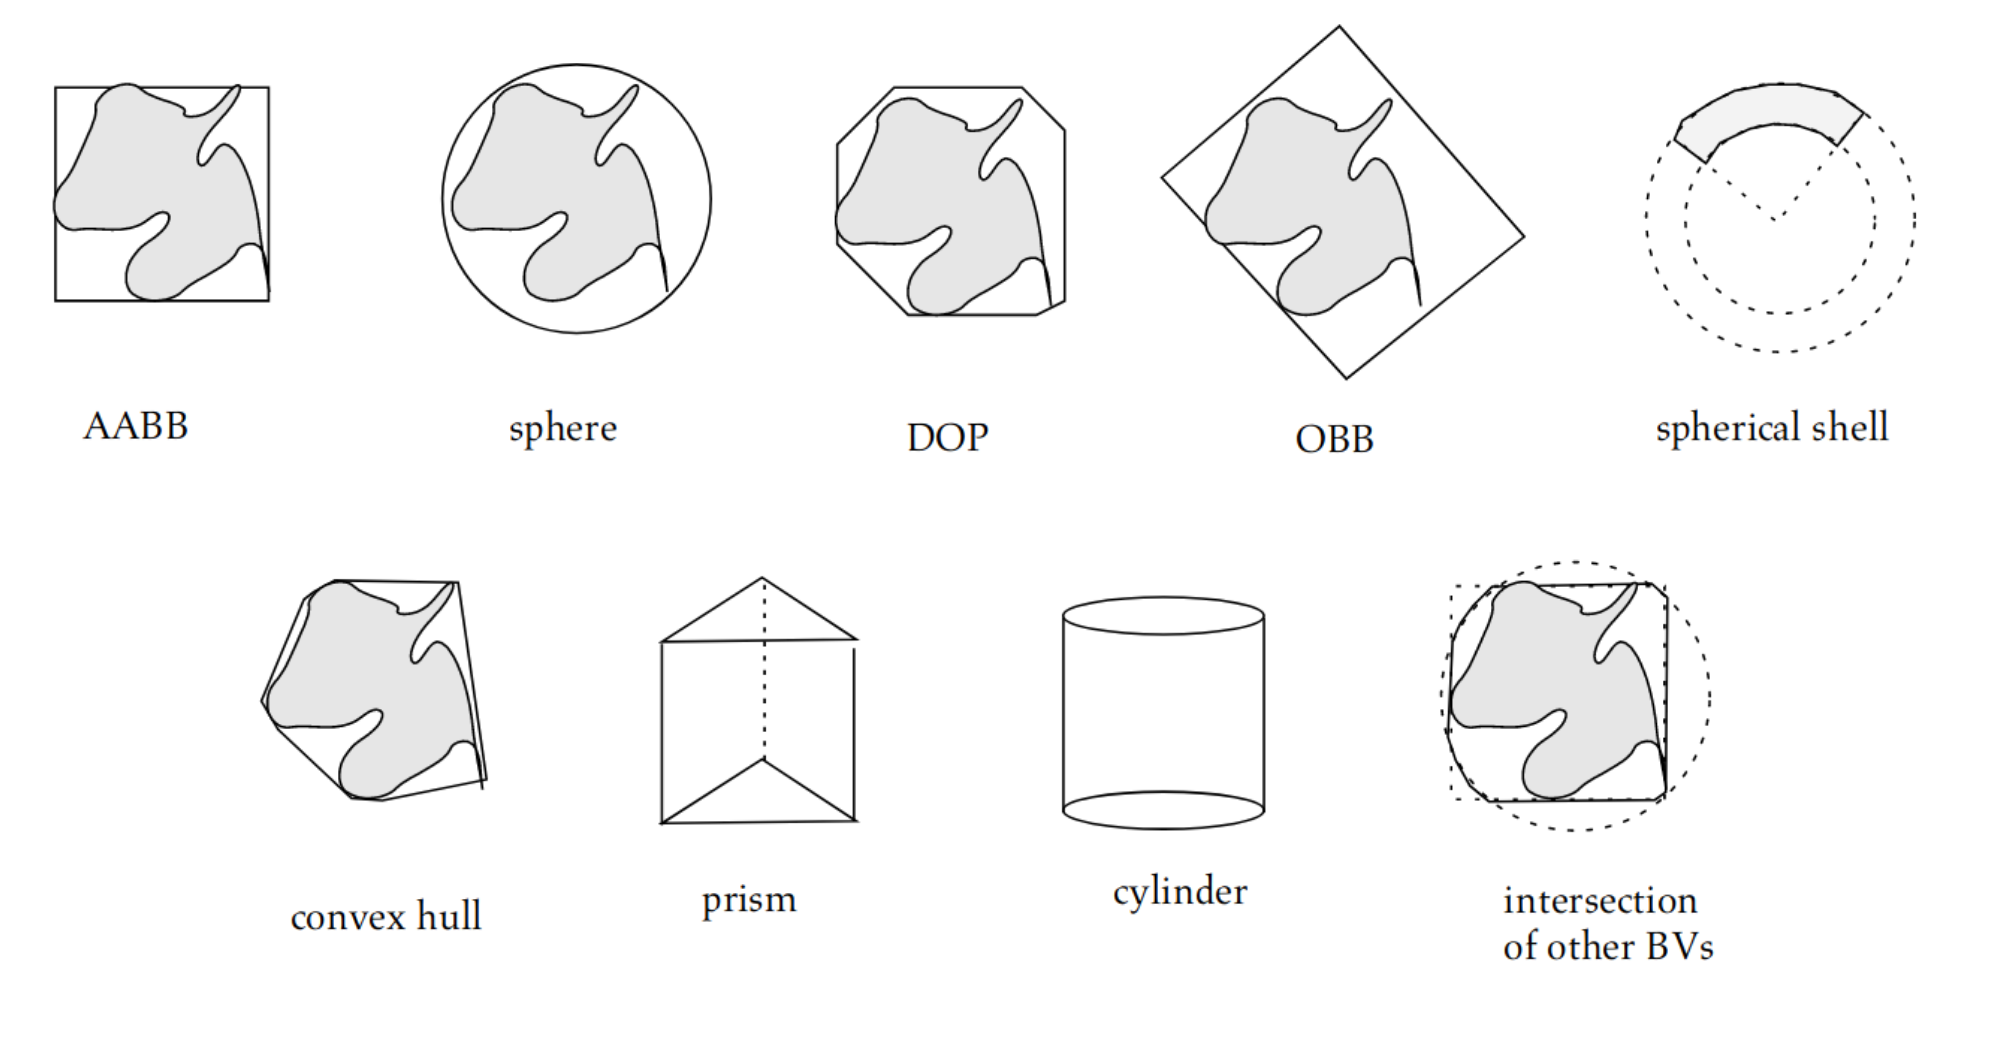
\includegraphics[width=0.9\linewidth]{images/bounding-volumes}
    \caption{Most commonly used bounding volumes. Source: \cite{gabriel_zachmann_geometric_2002}}
\end{figure}

To constrain the planes to the area where the points are located, a bounding volume can be used.
A bounding volume is a geometric shape that encloses a set of points or other shapes,
and is often used to simplify collision detection or culling~\cite{gabriel_zachmann_geometric_2002}.
In this case the bounding volume will be used to generate a mesh that represents the area where the points are located.
Common bounding volumes include axis-aligned bounding boxes (AABB), spheres, or oriented bounding boxes (OBB).
A more complex bounding volume is the convex hull, which is the smallest convex polygon that contains all the points~\cite{gabriel_zachmann_geometric_2002}.
A rubber band can be used to illustrate the concept: If a rubber band is stretched around a set of points represented by nails in a board,
the convex hull is the shape a rubber band takes when it is released, as illustrated in figure~\ref{fig:convex-hull}~\cite{de_berg_computational_2008}.
As the convex hull is the most accurate commonly used bounding volume,
it will be used for constraining the planes going forward.

\begin{figure}[ht!]
    \centering
    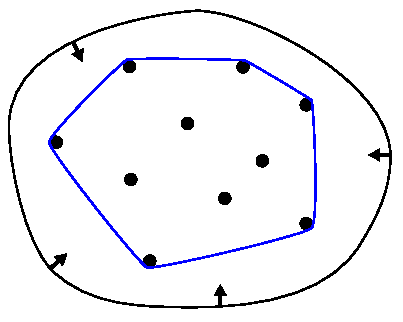
\includegraphics[width=0.25\linewidth]{images/ConvexHull}
    \caption{Rubber band analogy for the Convex Hull. Source: \href{https://commons.wikimedia.org/wiki/File:ConvexHull.svg}{Wikimedia Commons}}
\end{figure}

\subsubsection{Convex Hull Algorithms}
There are many algorithms available for calculating the convex hull, as it is a well-known problem in computational geometry.
This section will mainly cover the Graham Scan.
For a more comprehensive overview of available algorithms, see~\cite{de_berg_computational_2008} section 1.4.

In~\citeyear{graham_efficient_1972}~\cite{graham_efficient_1972} proposed an algorithm to calculate
the convex hull of $n$ points in $O(n \log n)$ time, the Graham's Scan.
The Graham scan algorithm begins by selecting the point with the lowest y-coordinate (or the leftmost point in the case of a tie).
Note that the original paper describes using the center of the points as the starting point,
but common implementations use the lowest y-coordinate
~\footfullcite{noauthor_graham_2024}\multiplefootnoteseparator\footfullcite{noauthor_convex_2013} --
the core concepts remain the same.
After selecting the starting points, it then sorts the remaining points in ascending order
of their polar angles relative to the starting point.
If two points have the same polar angle, only the farthest point is kept.
Finally, it iteratively considers each point in the sorted order and determines whether it
makes a clockwise or counterclockwise turn relative to the previous two points on the convex hull.
If it makes a clockwise, the algorithm removes the previous point from the convex hull
and repeats the process until all points have been considered.


\begin{figure}[h!]
    \centering
    \begin{subfigure}[b]{0.25\textwidth}
        \centering
        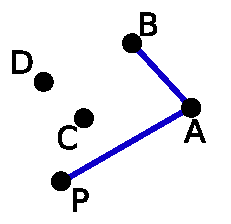
\includegraphics[width=0.9\linewidth]{images/graham1}
        \caption{$PAB$ are counterclockwise, $A$ is kept}
    \end{subfigure}%
    \hspace{0.05\textwidth} % Added space between subfigures
    \begin{subfigure}[b]{0.25\textwidth}
        \centering
        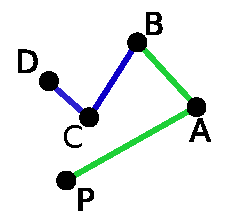
\includegraphics[width=0.9\linewidth]{images/graham2}
        \caption{$BCD$ are clockwise, $C$ is removed}
    \end{subfigure}%
    \hspace{0.05\textwidth} % Added space between subfigures
    \begin{subfigure}[b]{0.25\textwidth}
        \centering
        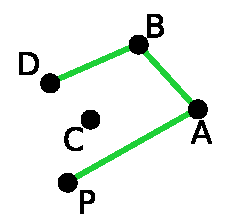
\includegraphics[width=0.9\linewidth]{images/graham3}
        \caption{$ABD$ are clockwise, $D$ is kept, resulting hull}
    \end{subfigure}%
    \caption{Example of the Graham Scan algorithm applied to a set of points. Source: \href{https://commons.wikimedia.org/wiki/File:Graham_Scan.svg}{Wikimedia Commons}}
    \label{fig:graham}
\end{figure}

\cite{andrew_another_1979} later proposed a variation of the algorithm called the
monotone chain in~\citeyear{andrew_another_1979}, which sorts the points by their
x-coordinate and y-coordinates instead of their polar angle.
It then constructs the upper and lower hulls separately, which are then merged to form the convex hull.


\begin{figure}[ht!]
    \centering
    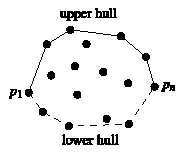
\includegraphics[width=0.35\linewidth]{images/andrews}
    \caption{Upper and lower hull of Andrew's monotone chain algorithm. Source:~\cite{de_berg_computational_2008}}
\end{figure}


%todo: Explain the algorithm

More recent algorithms like Chan's algorithm~\cite{chan_optimal_1996} combine the graham scan with other techniques to solve the problem in $O(n \log h)$ time,
where $h$ is the number of points of the convex hull.
Thus, in case $h$ is much smaller than $n$, these algorithms are faster than the Graham's Scan.

For the purpose of this thesis, the Chan's algorithm would be the most efficient choice,
as the number of points of the convex hull is expected to be much smaller than the total number of points.
However, as Chan's algorithm is more complex to implement and the performance of the convex hull algorithm
is small compared to running the RANSAC algorithm, Andrew's Monotone Chain Algorithm is used here instead.



\subsubsection{Rendering Planes Constrained by the Convex Hull}
To render a plane constrained by the convex hull,
a triangle mesh can be created with triangles consisting of two subsequent triangles of the hull vertices and the centroid of the hull as the third vertex each.
Figure~\ref{fig:convex-hull} shows the result of the convex hull algorithm implemented into the application.
Prior to detecting the planes, the smartphone has been moved around the scene to capture the points from different angles.

\begin{figure}[ht!]

    \centering
    \begin{subfigure}[b]{0.4\textwidth}
        \centering
        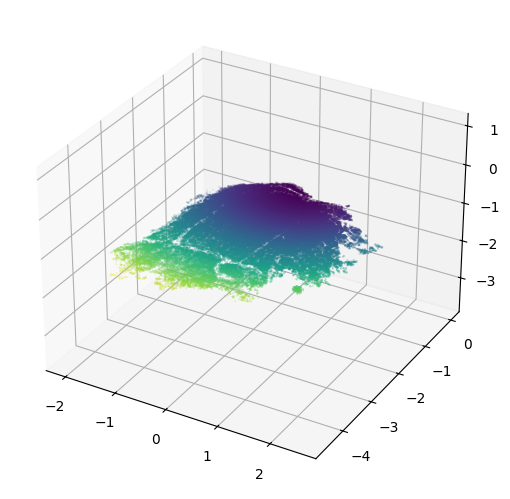
\includegraphics[width=\linewidth]{python/plots/hull/points}
        \caption{Point data}
    \end{subfigure}%
    \begin{subfigure}[b]{0.4\textwidth}
        \centering
        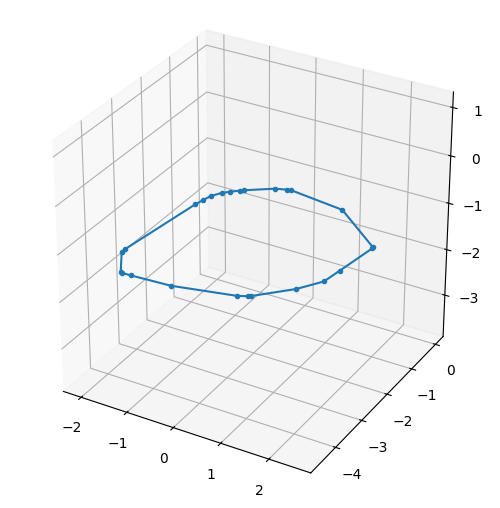
\includegraphics[width=\linewidth]{python/plots/hull/hull}
        \caption{Convex Hull}
    \end{subfigure}%

    \vspace{0.5em}

    \begin{subfigure}[b]{0.8\textwidth}
        \centering
        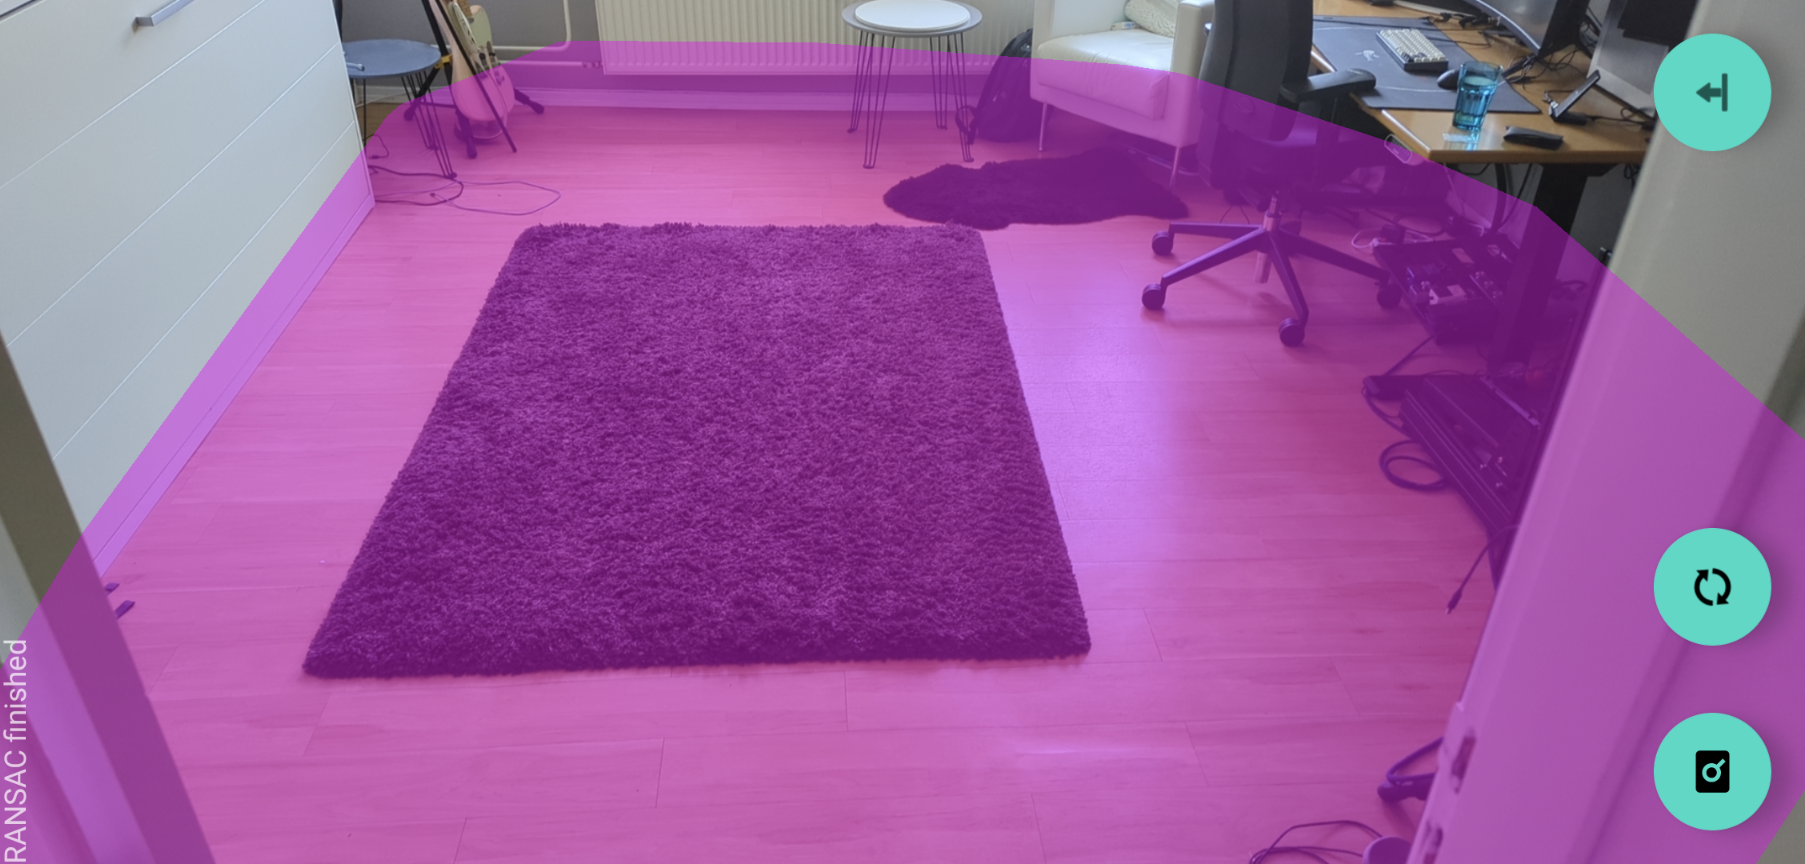
\includegraphics[width=\linewidth]{images/hull}
        \caption{Rendered Primitive}
    \end{subfigure}%
    \caption{Convex Hull with real data}
    \label{fig:convex-hull}
\end{figure}



%\section{User Interface of the Mobile Application}
%The application has a simple user interface, consisting of 3 buttons and one label that displays the current status,
%visible in figure~\ref{fig:convex-hull}.
%Capturing depth data will automatically start once tracking is initialized.
%The point cloud is then continuously updated with new depth data on each frame.
%The amount of captured points is displayed in the label.
%The user can then press the "Detect Planes" button to run the RANSAC algorithm on the point cloud.
%Once detection is complete, the detected planes are rendered on the screen.
%Another button allows the user reset the detection results and start over.
%The button on the right side of the screen allows the user to upload the constructed point cloud to a server, as will be discussed in section~\ref{sec:point-clouds}.